% Options for packages loaded elsewhere
\PassOptionsToPackage{unicode}{hyperref}
\PassOptionsToPackage{hyphens}{url}
\PassOptionsToPackage{dvipsnames,svgnames,x11names}{xcolor}
%
\documentclass[
  letterpaper,
  DIV=11,
  numbers=noendperiod]{scrartcl}

\usepackage{amsmath,amssymb}
\usepackage{iftex}
\ifPDFTeX
  \usepackage[T1]{fontenc}
  \usepackage[utf8]{inputenc}
  \usepackage{textcomp} % provide euro and other symbols
\else % if luatex or xetex
  \usepackage{unicode-math}
  \defaultfontfeatures{Scale=MatchLowercase}
  \defaultfontfeatures[\rmfamily]{Ligatures=TeX,Scale=1}
\fi
\usepackage{lmodern}
\ifPDFTeX\else  
    % xetex/luatex font selection
\fi
% Use upquote if available, for straight quotes in verbatim environments
\IfFileExists{upquote.sty}{\usepackage{upquote}}{}
\IfFileExists{microtype.sty}{% use microtype if available
  \usepackage[]{microtype}
  \UseMicrotypeSet[protrusion]{basicmath} % disable protrusion for tt fonts
}{}
\makeatletter
\@ifundefined{KOMAClassName}{% if non-KOMA class
  \IfFileExists{parskip.sty}{%
    \usepackage{parskip}
  }{% else
    \setlength{\parindent}{0pt}
    \setlength{\parskip}{6pt plus 2pt minus 1pt}}
}{% if KOMA class
  \KOMAoptions{parskip=half}}
\makeatother
\usepackage{xcolor}
\setlength{\emergencystretch}{3em} % prevent overfull lines
\setcounter{secnumdepth}{5}
% Make \paragraph and \subparagraph free-standing
\ifx\paragraph\undefined\else
  \let\oldparagraph\paragraph
  \renewcommand{\paragraph}[1]{\oldparagraph{#1}\mbox{}}
\fi
\ifx\subparagraph\undefined\else
  \let\oldsubparagraph\subparagraph
  \renewcommand{\subparagraph}[1]{\oldsubparagraph{#1}\mbox{}}
\fi

\usepackage{color}
\usepackage{fancyvrb}
\newcommand{\VerbBar}{|}
\newcommand{\VERB}{\Verb[commandchars=\\\{\}]}
\DefineVerbatimEnvironment{Highlighting}{Verbatim}{commandchars=\\\{\}}
% Add ',fontsize=\small' for more characters per line
\usepackage{framed}
\definecolor{shadecolor}{RGB}{241,243,245}
\newenvironment{Shaded}{\begin{snugshade}}{\end{snugshade}}
\newcommand{\AlertTok}[1]{\textcolor[rgb]{0.68,0.00,0.00}{#1}}
\newcommand{\AnnotationTok}[1]{\textcolor[rgb]{0.37,0.37,0.37}{#1}}
\newcommand{\AttributeTok}[1]{\textcolor[rgb]{0.40,0.45,0.13}{#1}}
\newcommand{\BaseNTok}[1]{\textcolor[rgb]{0.68,0.00,0.00}{#1}}
\newcommand{\BuiltInTok}[1]{\textcolor[rgb]{0.00,0.23,0.31}{#1}}
\newcommand{\CharTok}[1]{\textcolor[rgb]{0.13,0.47,0.30}{#1}}
\newcommand{\CommentTok}[1]{\textcolor[rgb]{0.37,0.37,0.37}{#1}}
\newcommand{\CommentVarTok}[1]{\textcolor[rgb]{0.37,0.37,0.37}{\textit{#1}}}
\newcommand{\ConstantTok}[1]{\textcolor[rgb]{0.56,0.35,0.01}{#1}}
\newcommand{\ControlFlowTok}[1]{\textcolor[rgb]{0.00,0.23,0.31}{#1}}
\newcommand{\DataTypeTok}[1]{\textcolor[rgb]{0.68,0.00,0.00}{#1}}
\newcommand{\DecValTok}[1]{\textcolor[rgb]{0.68,0.00,0.00}{#1}}
\newcommand{\DocumentationTok}[1]{\textcolor[rgb]{0.37,0.37,0.37}{\textit{#1}}}
\newcommand{\ErrorTok}[1]{\textcolor[rgb]{0.68,0.00,0.00}{#1}}
\newcommand{\ExtensionTok}[1]{\textcolor[rgb]{0.00,0.23,0.31}{#1}}
\newcommand{\FloatTok}[1]{\textcolor[rgb]{0.68,0.00,0.00}{#1}}
\newcommand{\FunctionTok}[1]{\textcolor[rgb]{0.28,0.35,0.67}{#1}}
\newcommand{\ImportTok}[1]{\textcolor[rgb]{0.00,0.46,0.62}{#1}}
\newcommand{\InformationTok}[1]{\textcolor[rgb]{0.37,0.37,0.37}{#1}}
\newcommand{\KeywordTok}[1]{\textcolor[rgb]{0.00,0.23,0.31}{#1}}
\newcommand{\NormalTok}[1]{\textcolor[rgb]{0.00,0.23,0.31}{#1}}
\newcommand{\OperatorTok}[1]{\textcolor[rgb]{0.37,0.37,0.37}{#1}}
\newcommand{\OtherTok}[1]{\textcolor[rgb]{0.00,0.23,0.31}{#1}}
\newcommand{\PreprocessorTok}[1]{\textcolor[rgb]{0.68,0.00,0.00}{#1}}
\newcommand{\RegionMarkerTok}[1]{\textcolor[rgb]{0.00,0.23,0.31}{#1}}
\newcommand{\SpecialCharTok}[1]{\textcolor[rgb]{0.37,0.37,0.37}{#1}}
\newcommand{\SpecialStringTok}[1]{\textcolor[rgb]{0.13,0.47,0.30}{#1}}
\newcommand{\StringTok}[1]{\textcolor[rgb]{0.13,0.47,0.30}{#1}}
\newcommand{\VariableTok}[1]{\textcolor[rgb]{0.07,0.07,0.07}{#1}}
\newcommand{\VerbatimStringTok}[1]{\textcolor[rgb]{0.13,0.47,0.30}{#1}}
\newcommand{\WarningTok}[1]{\textcolor[rgb]{0.37,0.37,0.37}{\textit{#1}}}

\providecommand{\tightlist}{%
  \setlength{\itemsep}{0pt}\setlength{\parskip}{0pt}}\usepackage{longtable,booktabs,array}
\usepackage{calc} % for calculating minipage widths
% Correct order of tables after \paragraph or \subparagraph
\usepackage{etoolbox}
\makeatletter
\patchcmd\longtable{\par}{\if@noskipsec\mbox{}\fi\par}{}{}
\makeatother
% Allow footnotes in longtable head/foot
\IfFileExists{footnotehyper.sty}{\usepackage{footnotehyper}}{\usepackage{footnote}}
\makesavenoteenv{longtable}
\usepackage{graphicx}
\makeatletter
\def\maxwidth{\ifdim\Gin@nat@width>\linewidth\linewidth\else\Gin@nat@width\fi}
\def\maxheight{\ifdim\Gin@nat@height>\textheight\textheight\else\Gin@nat@height\fi}
\makeatother
% Scale images if necessary, so that they will not overflow the page
% margins by default, and it is still possible to overwrite the defaults
% using explicit options in \includegraphics[width, height, ...]{}
\setkeys{Gin}{width=\maxwidth,height=\maxheight,keepaspectratio}
% Set default figure placement to htbp
\makeatletter
\def\fps@figure{htbp}
\makeatother

\KOMAoption{captions}{tableheading}
\makeatletter
\@ifpackageloaded{caption}{}{\usepackage{caption}}
\AtBeginDocument{%
\ifdefined\contentsname
  \renewcommand*\contentsname{Table of contents}
\else
  \newcommand\contentsname{Table of contents}
\fi
\ifdefined\listfigurename
  \renewcommand*\listfigurename{List of Figures}
\else
  \newcommand\listfigurename{List of Figures}
\fi
\ifdefined\listtablename
  \renewcommand*\listtablename{List of Tables}
\else
  \newcommand\listtablename{List of Tables}
\fi
\ifdefined\figurename
  \renewcommand*\figurename{Figure}
\else
  \newcommand\figurename{Figure}
\fi
\ifdefined\tablename
  \renewcommand*\tablename{Table}
\else
  \newcommand\tablename{Table}
\fi
}
\@ifpackageloaded{float}{}{\usepackage{float}}
\floatstyle{ruled}
\@ifundefined{c@chapter}{\newfloat{codelisting}{h}{lop}}{\newfloat{codelisting}{h}{lop}[chapter]}
\floatname{codelisting}{Stan

Program}
\newcommand*\listoflistings{\listof{codelisting}{List of Listings}}
\makeatother
\makeatletter
\makeatother
\makeatletter
\@ifpackageloaded{caption}{}{\usepackage{caption}}
\@ifpackageloaded{subcaption}{}{\usepackage{subcaption}}
\makeatother
\ifLuaTeX
  \usepackage{selnolig}  % disable illegal ligatures
\fi
\usepackage{bookmark}

\IfFileExists{xurl.sty}{\usepackage{xurl}}{} % add URL line breaks if available
\urlstyle{same} % disable monospaced font for URLs
\hypersetup{
  pdftitle={Generative Modeling of Customer Conversion},
  pdfauthor={Michael Betancourt},
  colorlinks=true,
  linkcolor={blue},
  filecolor={Maroon},
  citecolor={Blue},
  urlcolor={Blue},
  pdfcreator={LaTeX via pandoc}}

\title{Generative Modeling of Customer Conversion}
\author{Michael Betancourt}
\date{July 2024}

\begin{document}
\maketitle

\renewcommand*\contentsname{Table of contents}
{
\hypersetup{linkcolor=}
\setcounter{tocdepth}{3}
\tableofcontents
}
In this short case study I demonstrate narratively modeling by
implementing the conceptual analysis discussed in Section 3.3 of my much
more comprehensive
\href{https://betanalpha.github.io/assets/case_studies/generative_modeling.html}{discussion
of the subject}. If you are just getting started with the topic then I
recommend first reviewing my chapters on
\href{https://betanalpha.github.io/assets/case_studies/modeling_and_inference.html}{probabilistic
modeling and Bayesian inference},
\href{https://betanalpha.github.io/assets/case_studies/stan_intro.html}{Stan},
and
\href{https://betanalpha.github.io/assets/case_studies/principled_bayesian_workflow.html}{model
critique and iterative model development}.

\section{The Conceptual Data Generating
Process}\label{the-conceptual-data-generating-process}

The basis of narratively generative modeling is domain expertise. We
cannot model a data generating process unless we know something about
its possible behaviors!

Moreover we all have our own experiences and none of us share exactly
the same domain expertise. An immediate consequence of this diversity is
that there is no universal application that resonates with everyone's
domain expertise. To make this case study as broadly accessible as
possible I will consider an abstract marketing example and simply
provide the relevant domain expertise whenever it is necessary.

With all of that said let's say that we are interested in how often
people who engage with a business end up \emph{converting} to some
deeper engagement. For example we might be curious about how likely
someone who is exposed to an advertisement for a business is to visit a
physical location of that business. Alternatively we might be more
concerned with how likely someone who visits a visits a physical
location is to buy any item or even a particular item, or how likely
someone who has made a purchase previously is to make a future purchase.
Similarly we might be interested in how likely someone who browses a
website is to signup for a mailing list, download a piece of software,
and the like.

These interactions between a potential customer and a business motivate
a relatively straightforward data generating process. Because a
conversion is either made or not individual interactions result in a
binary outcome \[
y \in \{0, 1\}
\] where \(1\) denotes a conversion and \(0\) denotes no conversion. Any
compatible data generating process is then responsible for defining the
probability of these outcomes.

Now the probability of conversion is a complicated object. Conceptually
it will depend on the behavior of each visitor, the behavior of the
business with which they engage, and the details of that engagement. The
possibilities can quickly become overwhelming. We can always make the
modeling more manageable, however, by starting as simple as possible.

Before that, however, let's set up our computing environment and take a
look at the available data.

\section{Computational Environment
Setup}\label{computational-environment-setup}

Here we'll be using \texttt{R} with the base graphics cleaned up a bit.

\begin{Shaded}
\begin{Highlighting}[]
\FunctionTok{par}\NormalTok{(}\AttributeTok{family=}\StringTok{"serif"}\NormalTok{, }\AttributeTok{las=}\DecValTok{1}\NormalTok{, }\AttributeTok{bty=}\StringTok{"l"}\NormalTok{,}
    \AttributeTok{cex.axis=}\DecValTok{1}\NormalTok{, }\AttributeTok{cex.lab=}\DecValTok{1}\NormalTok{, }\AttributeTok{cex.main=}\DecValTok{1}\NormalTok{,}
    \AttributeTok{xaxs=}\StringTok{"i"}\NormalTok{, }\AttributeTok{yaxs=}\StringTok{"i"}\NormalTok{, }\AttributeTok{mar =} \FunctionTok{c}\NormalTok{(}\DecValTok{5}\NormalTok{, }\DecValTok{5}\NormalTok{, }\DecValTok{3}\NormalTok{, }\DecValTok{5}\NormalTok{))}
\end{Highlighting}
\end{Shaded}

Next we'll load \texttt{Stan} and configure a few settings.

\begin{Shaded}
\begin{Highlighting}[]
\FunctionTok{library}\NormalTok{(rstan)}
\FunctionTok{rstan\_options}\NormalTok{(}\AttributeTok{auto\_write =} \ConstantTok{TRUE}\NormalTok{)            }\CommentTok{\# Cache compiled Stan programs}
\FunctionTok{options}\NormalTok{(}\AttributeTok{mc.cores =}\NormalTok{ parallel}\SpecialCharTok{::}\FunctionTok{detectCores}\NormalTok{()) }\CommentTok{\# Parallelize chains}
\NormalTok{parallel}\SpecialCharTok{:::}\FunctionTok{setDefaultClusterOptions}\NormalTok{(}\AttributeTok{setup\_strategy =} \StringTok{"sequential"}\NormalTok{)}
\end{Highlighting}
\end{Shaded}

Finally we'll load some utility functions into a local environment to
facilitate the implementation of Bayesian inference.

\begin{Shaded}
\begin{Highlighting}[]
\NormalTok{util }\OtherTok{\textless{}{-}} \FunctionTok{new.env}\NormalTok{()}
\end{Highlighting}
\end{Shaded}

First is a suite Markov chain Monte Carlo diagnostics and estimation
tools; this code and supporting documentation are both available on
\href{https://github.com/betanalpha/mcmc_diagnostics}{GitHub}.

\begin{Shaded}
\begin{Highlighting}[]
\FunctionTok{source}\NormalTok{(}\StringTok{\textquotesingle{}mcmc\_visualization\_tools.R\textquotesingle{}}\NormalTok{, }\AttributeTok{local=}\NormalTok{util)}
\end{Highlighting}
\end{Shaded}

Second is a suite of posterior and posterior predictive visualization
functions based on Markov chain Monte Carlo estimation. Again the code
and supporting documentation are available on
\href{https://github.com/betanalpha/mcmc_visualization_tools}{GitHub}.

\begin{Shaded}
\begin{Highlighting}[]
\FunctionTok{source}\NormalTok{(}\StringTok{\textquotesingle{}mcmc\_analysis\_tools\_rstan.R\textquotesingle{}}\NormalTok{, }\AttributeTok{local=}\NormalTok{util)}
\end{Highlighting}
\end{Shaded}

\section{Data Exploration}\label{data-exploration}

With our environment sorted let's load in the available data which
consists of two arrays, each of size \texttt{N\ =\ 1500}.

\begin{Shaded}
\begin{Highlighting}[]
\NormalTok{data }\OtherTok{\textless{}{-}} \FunctionTok{read\_rdump}\NormalTok{(}\StringTok{\textquotesingle{}data/logs.data.R\textquotesingle{}}\NormalTok{)}

\FunctionTok{names}\NormalTok{(data)}
\end{Highlighting}
\end{Shaded}

\begin{verbatim}
[1] "x" "y" "N"
\end{verbatim}

The array variable \texttt{y} contains the conversion outcomes of
previous engagements, with successful conversions coded as a \(1\) and
unsuccessful conversions coded as a \(0\). Overall there are a bit more
failures than successes.

\begin{Shaded}
\begin{Highlighting}[]
\FunctionTok{table}\NormalTok{(data}\SpecialCharTok{$}\NormalTok{y)}
\end{Highlighting}
\end{Shaded}

\begin{verbatim}

  0   1 
859 641 
\end{verbatim}

We also have access to the array variable \texttt{x} which contains the
total purchases that each customer has made, in United States Dollar or
USD, prior to the observed engagement. Most customers have spent a
moderate amount with a decaying tail of more prolific shoppers.

\begin{Shaded}
\begin{Highlighting}[]
\FunctionTok{par}\NormalTok{(}\AttributeTok{mfrow=}\FunctionTok{c}\NormalTok{(}\DecValTok{1}\NormalTok{, }\DecValTok{1}\NormalTok{), }\AttributeTok{mar=}\FunctionTok{c}\NormalTok{(}\DecValTok{5}\NormalTok{, }\DecValTok{5}\NormalTok{, }\DecValTok{1}\NormalTok{, }\DecValTok{1}\NormalTok{))}

\NormalTok{util}\SpecialCharTok{$}\FunctionTok{plot\_line\_hist}\NormalTok{(data}\SpecialCharTok{$}\NormalTok{x, }\AttributeTok{xlab=}\StringTok{"Previous Purchases (USD)"}\NormalTok{)}
\end{Highlighting}
\end{Shaded}

\includegraphics{customer_conversion_files/figure-pdf/unnamed-chunk-9-1.pdf}

Interestingly no customers have zero prior purchases, indicating that
our data set consistent entirely of repeat customers. This limits what
we might be able to learn about entirely new customers.

\begin{Shaded}
\begin{Highlighting}[]
\FunctionTok{par}\NormalTok{(}\AttributeTok{mfrow=}\FunctionTok{c}\NormalTok{(}\DecValTok{1}\NormalTok{, }\DecValTok{1}\NormalTok{), }\AttributeTok{mar=}\FunctionTok{c}\NormalTok{(}\DecValTok{5}\NormalTok{, }\DecValTok{5}\NormalTok{, }\DecValTok{1}\NormalTok{, }\DecValTok{1}\NormalTok{))}

\NormalTok{util}\SpecialCharTok{$}\FunctionTok{plot\_line\_hist}\NormalTok{(data}\SpecialCharTok{$}\NormalTok{x, }\DecValTok{0}\NormalTok{, }\DecValTok{10}\NormalTok{, }\DecValTok{1}\NormalTok{, }\AttributeTok{xlab=}\StringTok{"Previous Purchases (USD)"}\NormalTok{)}
\end{Highlighting}
\end{Shaded}

\begin{verbatim}
Warning in check_bin_containment(bin_min, bin_max, values): 1494 values (99.6%)
fell above the binning.
\end{verbatim}

\includegraphics{customer_conversion_files/figure-pdf/unnamed-chunk-10-1.pdf}

The availability of data beyond just the conversion outcomes allows us
to consider more sophisticated data generating processes. In particular
we can consider not just the aggregate conversion probability but also
the conversion probability conditional on the previous purchases. Just
by looking at the data we can see that this relationship is not trivial.

\begin{Shaded}
\begin{Highlighting}[]
\FunctionTok{par}\NormalTok{(}\AttributeTok{mfrow=}\FunctionTok{c}\NormalTok{(}\DecValTok{1}\NormalTok{, }\DecValTok{1}\NormalTok{), }\AttributeTok{mar=}\FunctionTok{c}\NormalTok{(}\DecValTok{5}\NormalTok{, }\DecValTok{5}\NormalTok{, }\DecValTok{1}\NormalTok{, }\DecValTok{1}\NormalTok{))}

\NormalTok{bins }\OtherTok{\textless{}{-}} \FunctionTok{seq}\NormalTok{(}\DecValTok{0}\NormalTok{, }\DecValTok{6100}\NormalTok{, }\DecValTok{305}\NormalTok{)}
\NormalTok{B }\OtherTok{\textless{}{-}} \FunctionTok{length}\NormalTok{(bins) }\SpecialCharTok{{-}} \DecValTok{1}

\NormalTok{idxs }\OtherTok{\textless{}{-}} \FunctionTok{rep}\NormalTok{(}\DecValTok{1}\SpecialCharTok{:}\NormalTok{B, }\AttributeTok{each=}\DecValTok{2}\NormalTok{)}
\NormalTok{xs }\OtherTok{\textless{}{-}} \FunctionTok{sapply}\NormalTok{(}\DecValTok{1}\SpecialCharTok{:}\FunctionTok{length}\NormalTok{(idxs),}
             \ControlFlowTok{function}\NormalTok{(b) }\ControlFlowTok{if}\NormalTok{(b }\SpecialCharTok{\%\%} \DecValTok{2} \SpecialCharTok{==} \DecValTok{1}\NormalTok{) bins[idxs[b]]}
                         \ControlFlowTok{else}\NormalTok{            bins[idxs[b] }\SpecialCharTok{+} \DecValTok{1}\NormalTok{])}

\NormalTok{binned\_freqs }\OtherTok{\textless{}{-}} \FunctionTok{sapply}\NormalTok{(}\DecValTok{1}\SpecialCharTok{:}\NormalTok{B, }\ControlFlowTok{function}\NormalTok{(b)}
                       \FunctionTok{mean}\NormalTok{(data}\SpecialCharTok{$}\NormalTok{y[bins[b] }\SpecialCharTok{\textless{}}\NormalTok{ data}\SpecialCharTok{$}\NormalTok{x }\SpecialCharTok{\&}\NormalTok{ data}\SpecialCharTok{$}\NormalTok{x }\SpecialCharTok{\textless{}=}\NormalTok{ bins[b }\SpecialCharTok{+} \DecValTok{1}\NormalTok{]]))}
\NormalTok{binned\_freqs }\OtherTok{\textless{}{-}} \FunctionTok{rep}\NormalTok{(binned\_freqs, }\AttributeTok{each=}\DecValTok{2}\NormalTok{)}

\FunctionTok{plot}\NormalTok{(xs, binned\_freqs, }\AttributeTok{type=}\StringTok{"l"}\NormalTok{, }\AttributeTok{lwd=}\DecValTok{2}\NormalTok{,}
     \AttributeTok{xlab=}\StringTok{"Previous Purchases (USD)"}\NormalTok{,}
     \AttributeTok{ylab=}\StringTok{"Binned Conversion Frequencies"}\NormalTok{)}
\end{Highlighting}
\end{Shaded}

\includegraphics{customer_conversion_files/figure-pdf/unnamed-chunk-11-1.pdf}

\section{Modeling}\label{modeling}

Having reasoned through our domain expertise and explored the available
data we are finally ready to consider modeling the relevant data
generating process. In order to avoid being overwhelmed by the potential
complexities we will start simple and then iteratively incorporate more
complexity based on the posterior retrodictive performance of each
model.

\subsection{Model 1}\label{model-1}

If we assume that all customers behave identically and ignore the
previous purchases altogether then we can model the aggregate conversion
outcomes with a Bernoulli observational model parameterized by a single
probability parameter \(\theta\), \[
\pi(y_{1}, \ldots, y_{N} \mid \theta)
=
\prod_{n = 1}^{N} \text{Bernoulli} \,(y_{n} \mid \theta).
\]

Any available domain expertise about the reasonable behaviors in this
data generating process informs a prior model for \(\theta\). For
example if we are confident that the true conversion probability is less
than \(0.5\) then we could define a prior model with a beta probability
density function that contains \(99\%\) of the prior probability to the
interval \(0 \le \theta \le 0.5\).

\begin{Shaded}
\begin{Highlighting}[]
\FunctionTok{par}\NormalTok{(}\AttributeTok{mfrow=}\FunctionTok{c}\NormalTok{(}\DecValTok{1}\NormalTok{, }\DecValTok{1}\NormalTok{), }\AttributeTok{mar=}\FunctionTok{c}\NormalTok{(}\DecValTok{5}\NormalTok{, }\DecValTok{5}\NormalTok{, }\DecValTok{1}\NormalTok{, }\DecValTok{1}\NormalTok{))}

\NormalTok{xs }\OtherTok{\textless{}{-}} \FunctionTok{seq}\NormalTok{(}\DecValTok{0}\NormalTok{, }\DecValTok{1}\NormalTok{, }\FloatTok{0.001}\NormalTok{)}
\FunctionTok{plot}\NormalTok{(xs, }\FunctionTok{dbeta}\NormalTok{(xs, }\FloatTok{0.5}\NormalTok{, }\FloatTok{5.0}\NormalTok{), }\AttributeTok{type=}\StringTok{"l"}\NormalTok{, }\AttributeTok{lwd=}\DecValTok{2}\NormalTok{, }\AttributeTok{col=}\NormalTok{util}\SpecialCharTok{$}\NormalTok{c\_mid\_teal)}
\end{Highlighting}
\end{Shaded}

\includegraphics{customer_conversion_files/figure-pdf/unnamed-chunk-12-1.pdf}

For more on containment prior modeling strategies see Section 3 of my
\href{https://betanalpha.github.io/assets/case_studies/prior_modeling.html}{prior
modeling chapter}.

The prior model then lifts the observational model into a full Bayesian
model \begin{align*}
\pi(y_{1}, \ldots, y_{N}, \theta)
&=
\pi(y_{1}, \ldots, y_{N} \mid \theta) \, \pi(\theta)
\\
&=
\left[ \prod_{n = 1}^{N} \pi(y_{n} \mid \theta) \right] \,
\pi(\theta)
\\
&=
\left[ \prod_{n = 1}^{N} \text{Bernoulli} \,(y_{n} \mid \theta) \right] \,
\pi(\theta).
\end{align*} We can also visualize the conditional structure of this
full Bayesian model with a directed graph (Figure~\ref{fig-model1}). For
an introduction to directed graphs as representations of probability
distributions see Section 4 of my chapter on
\href{https://betanalpha.github.io/assets/case_studies/probability_on_product_spaces.html\#4_Directed_Graphical_Models}{probability
theory on product spaces}.

\begin{figure}

\centering{

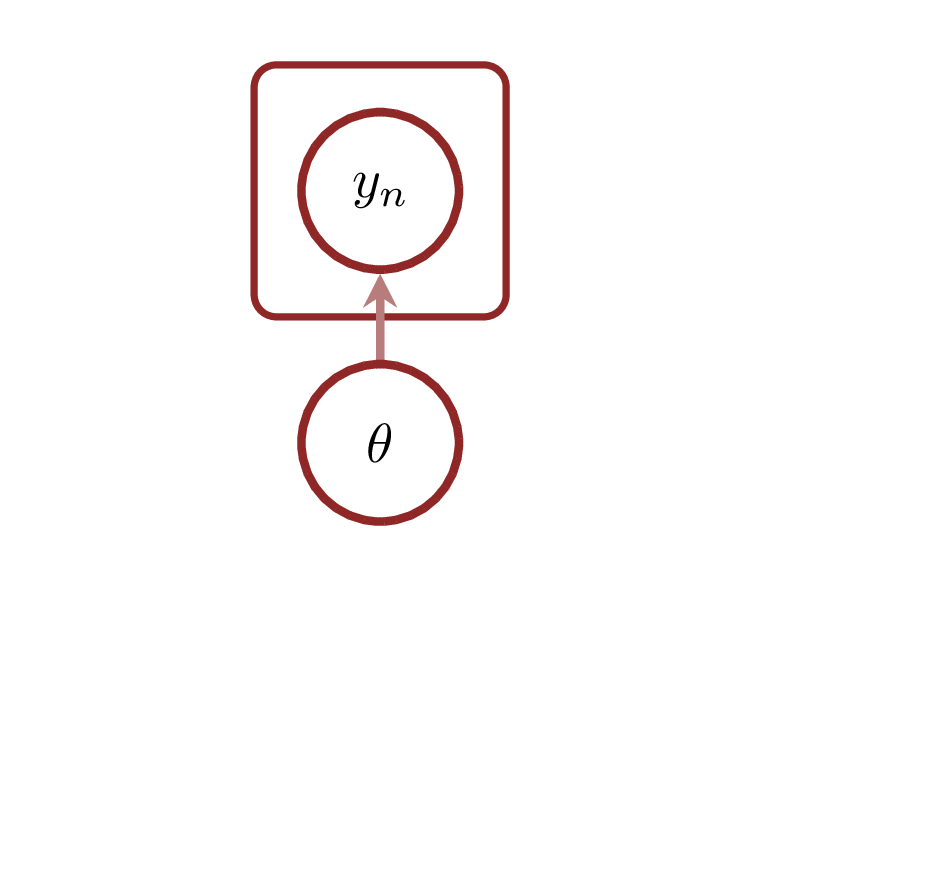
\includegraphics[width=0.5\textwidth,height=\textheight]{figures/1/1.png}

}

\caption{\label{fig-model1}Our first model of customer conversion
assumes that all customers behave the same, allowing their behavior to
be captured in a single probability parameter \(\theta\).}

\end{figure}%

To evaluate this full Bayesian model on the observed data and extract
posterior insights we will implement it as a probabilistic program in
the \texttt{Stan} modeling language. In addition to the full Bayesian
model we also implement posterior predictions in the
\texttt{generated\ quantities} block. Note that I am focusing on
explicitness and clarity in this Stan program and those that follow;
consequently these programs will not always demonstrate coding
techniques for optimal performance.

\begin{codelisting}

\caption{\texttt{model1.stan}}

\begin{Shaded}
\begin{Highlighting}[]
\KeywordTok{data}\NormalTok{ \{}
  \CommentTok{// Observed data}
  \DataTypeTok{int}\NormalTok{\textless{}}\KeywordTok{lower}\NormalTok{=}\DecValTok{1}\NormalTok{\textgreater{} N;                   }\CommentTok{// Number of unique visits}
  \DataTypeTok{array}\NormalTok{[N] }\DataTypeTok{int}\NormalTok{\textless{}}\KeywordTok{lower}\NormalTok{=}\DecValTok{0}\NormalTok{, }\KeywordTok{upper}\NormalTok{=}\DecValTok{1}\NormalTok{\textgreater{} y; }\CommentTok{// Conversion indicator}
\NormalTok{\}}

\KeywordTok{parameters}\NormalTok{ \{}
  \DataTypeTok{real}\NormalTok{\textless{}}\KeywordTok{lower}\NormalTok{=}\DecValTok{0}\NormalTok{, }\KeywordTok{upper}\NormalTok{=}\DecValTok{1}\NormalTok{\textgreater{} theta; }\CommentTok{// Conversion probability}
\NormalTok{\}}

\KeywordTok{model}\NormalTok{ \{}
  \CommentTok{// Prior model}
\NormalTok{  theta \textasciitilde{} beta(}\FloatTok{0.5}\NormalTok{, }\FloatTok{5.0}\NormalTok{); }\CommentTok{// 0 \textless{}\textasciitilde{} theta \textless{}\textasciitilde{} 0.5}

  \CommentTok{// Observational model}
  \ControlFlowTok{for}\NormalTok{ (n }\ControlFlowTok{in} \DecValTok{1}\NormalTok{:N) \{}
    \KeywordTok{target +=}\NormalTok{ bernoulli\_lpmf(y[n] | theta);}
\NormalTok{  \}}
\NormalTok{\}}

\KeywordTok{generated quantities}\NormalTok{ \{}
  \CommentTok{// Posterior predictions}
  \DataTypeTok{array}\NormalTok{[N] }\DataTypeTok{real}\NormalTok{ y\_pred;}
  \DataTypeTok{real}\NormalTok{ p\_hat\_pred;}

  \ControlFlowTok{for}\NormalTok{ (n }\ControlFlowTok{in} \DecValTok{1}\NormalTok{:N) \{}
\NormalTok{    y\_pred[n] = bernoulli\_rng(theta);}
\NormalTok{  \}}
\NormalTok{  p\_hat\_pred = mean(y\_pred);}
\NormalTok{\}}
\end{Highlighting}
\end{Shaded}

\end{codelisting}

We can then use the dynamic Hamiltonian Monte Carlo sampler in
\texttt{Stan} to quantify the behavior of the posterior distribution.

\begin{Shaded}
\begin{Highlighting}[]
\NormalTok{fit }\OtherTok{\textless{}{-}} \FunctionTok{stan}\NormalTok{(}\AttributeTok{file=}\StringTok{"stan\_programs/model1.stan"}\NormalTok{,}
            \AttributeTok{data=}\NormalTok{data, }\AttributeTok{seed=}\DecValTok{8438338}\NormalTok{,}
            \AttributeTok{warmup=}\DecValTok{1000}\NormalTok{, }\AttributeTok{iter=}\DecValTok{2024}\NormalTok{, }\AttributeTok{refresh=}\DecValTok{0}\NormalTok{)}
\end{Highlighting}
\end{Shaded}

Before examining the posterior output we need to check for any
indications that our computation is inaccurate. Fortunately there are no
signs of unfaithful posterior quantification here.

\begin{Shaded}
\begin{Highlighting}[]
\NormalTok{diagnostics1 }\OtherTok{\textless{}{-}}\NormalTok{ util}\SpecialCharTok{$}\FunctionTok{extract\_hmc\_diagnostics}\NormalTok{(fit)}
\NormalTok{util}\SpecialCharTok{$}\FunctionTok{check\_all\_hmc\_diagnostics}\NormalTok{(diagnostics1)}
\end{Highlighting}
\end{Shaded}

\begin{verbatim}
  All Hamiltonian Monte Carlo diagnostics are consistent with reliable
Markov chain Monte Carlo.
\end{verbatim}

\begin{Shaded}
\begin{Highlighting}[]
\NormalTok{samples1 }\OtherTok{\textless{}{-}}\NormalTok{ util}\SpecialCharTok{$}\FunctionTok{extract\_expectands}\NormalTok{(fit)}
\NormalTok{base\_samples }\OtherTok{\textless{}{-}}\NormalTok{ util}\SpecialCharTok{$}\FunctionTok{filter\_expectands}\NormalTok{(samples1, }\FunctionTok{c}\NormalTok{(}\StringTok{\textquotesingle{}theta\textquotesingle{}}\NormalTok{))}
\NormalTok{util}\SpecialCharTok{$}\FunctionTok{check\_all\_expectand\_diagnostics}\NormalTok{(base\_samples)}
\end{Highlighting}
\end{Shaded}

\begin{verbatim}
All expectands checked appear to be behaving well enough for reliable
Markov chain Monte Carlo estimation.
\end{verbatim}

Next we need to evaluate the adequacy of our modeling assumptions with
posterior retrodictive checks. Posterior retrodictive checks compare the
behavior of the observed data to the behavior of the posterior
predictive distribution for any inconsistencies. For much more on visual
posterior retrodictive checks see Section 1.4.3 of my
\href{https://betanalpha.github.io/assets/case_studies/principled_bayesian_workflow.html\#143_Posterior_Retrodiction_Checks}{iterative
model development chapter}.

Let's first consider retrodictive performance within the scope of the
empirical conversion frequency summary statistic that maps all
\(N = 1500\) binary outcomes to a single real-valued outcome, \[
\hat{p}(y_{1}, \ldots, y_{N}) = \frac{ \sum_{n = 1}^{N} y_{n} }{ N }.
\] Fortunately everything looks consistent.

\begin{Shaded}
\begin{Highlighting}[]
\FunctionTok{par}\NormalTok{(}\AttributeTok{mfrow=}\FunctionTok{c}\NormalTok{(}\DecValTok{1}\NormalTok{, }\DecValTok{1}\NormalTok{), }\AttributeTok{mar=}\FunctionTok{c}\NormalTok{(}\DecValTok{5}\NormalTok{, }\DecValTok{5}\NormalTok{, }\DecValTok{1}\NormalTok{, }\DecValTok{1}\NormalTok{))}

\NormalTok{util}\SpecialCharTok{$}\FunctionTok{plot\_expectand\_pushforward}\NormalTok{(samples1[[}\StringTok{\textquotesingle{}p\_hat\_pred\textquotesingle{}}\NormalTok{]], }\DecValTok{20}\NormalTok{,}
                                \AttributeTok{display\_name=}\StringTok{"Aggregate Conversion Frequency"}\NormalTok{,}
                                \AttributeTok{baseline=}\FunctionTok{mean}\NormalTok{(data}\SpecialCharTok{$}\NormalTok{y))}
\end{Highlighting}
\end{Shaded}

\includegraphics{customer_conversion_files/figure-pdf/unnamed-chunk-15-1.pdf}

Next we can explore how consistent the observed outcomes and posterior
predictive outcomes are in bins of previous purchases. The statistic
needed for this check is a bit more complicated; see Section 2.5 of my
\href{https://betanalpha.github.io/assets/case_studies/taylor_models.html\#25_Posterior_Retrodictive_Checks}{Taylor
modeling chapter} for a detailed construction.

The posterior predictive behavior concentrates around the same point in
all of the previous purchases bins. In hindsight this is unsurprising
given our simple model assumptions. On the other hand the observed data
exhibits a nontrivial relationship between conversion frequency and
previous purchases. In particular the disagreement extends beyond the
posterior predictive uncertainties, suggesting that our model is not
flexible enough to capture the true data generating behavior.

\begin{Shaded}
\begin{Highlighting}[]
\FunctionTok{par}\NormalTok{(}\AttributeTok{mfrow=}\FunctionTok{c}\NormalTok{(}\DecValTok{1}\NormalTok{, }\DecValTok{1}\NormalTok{), }\AttributeTok{mar=}\FunctionTok{c}\NormalTok{(}\DecValTok{5}\NormalTok{, }\DecValTok{5}\NormalTok{, }\DecValTok{1}\NormalTok{, }\DecValTok{1}\NormalTok{))}

\NormalTok{pred\_names }\OtherTok{\textless{}{-}} \FunctionTok{sapply}\NormalTok{(}\DecValTok{1}\SpecialCharTok{:}\NormalTok{data}\SpecialCharTok{$}\NormalTok{N, }\ControlFlowTok{function}\NormalTok{(n) }\FunctionTok{paste0}\NormalTok{(}\StringTok{\textquotesingle{}y\_pred[\textquotesingle{}}\NormalTok{, n, }\StringTok{\textquotesingle{}]\textquotesingle{}}\NormalTok{))}
\NormalTok{util}\SpecialCharTok{$}\FunctionTok{plot\_conditional\_mean\_quantiles}\NormalTok{(samples1, pred\_names, data}\SpecialCharTok{$}\NormalTok{x,}
                                     \DecValTok{0}\NormalTok{, }\DecValTok{6120}\NormalTok{, }\DecValTok{153}\NormalTok{,}
                                     \AttributeTok{baseline\_values=}\NormalTok{data}\SpecialCharTok{$}\NormalTok{y,}
                                     \AttributeTok{xlab=}\StringTok{"Previous Purchases (USD)"}\NormalTok{,}
                                     \AttributeTok{ylab=}\StringTok{"Binned Conversion Frequency"}\NormalTok{)}
\end{Highlighting}
\end{Shaded}

\includegraphics{customer_conversion_files/figure-pdf/unnamed-chunk-16-1.pdf}

At this point we \emph{could} examine posterior inferences, but we have
to be careful with their interpretation. Models that are too rigid often
contort themselves in order to accommodate as much as possible the
particular idiosyncrasies of the observed data, pulling the individual
parameters away from any generalizeable interpretation.

Interestingly we see here that the posterior distribution for \(\theta\)
is pushing up against our prior model which could be a sign that the
prior model is offering some regularization against this kind of
contortion.

\begin{Shaded}
\begin{Highlighting}[]
\FunctionTok{par}\NormalTok{(}\AttributeTok{mfrow=}\FunctionTok{c}\NormalTok{(}\DecValTok{1}\NormalTok{, }\DecValTok{1}\NormalTok{), }\AttributeTok{mar=}\FunctionTok{c}\NormalTok{(}\DecValTok{5}\NormalTok{, }\DecValTok{5}\NormalTok{, }\DecValTok{1}\NormalTok{, }\DecValTok{1}\NormalTok{))}

\NormalTok{util}\SpecialCharTok{$}\FunctionTok{plot\_expectand\_pushforward}\NormalTok{(samples1[[}\StringTok{\textquotesingle{}theta\textquotesingle{}}\NormalTok{]], }\DecValTok{100}\NormalTok{,}
                                \AttributeTok{display\_name=}\StringTok{"theta"}\NormalTok{,}
                                \AttributeTok{flim=}\FunctionTok{c}\NormalTok{(}\DecValTok{0}\NormalTok{, }\DecValTok{1}\NormalTok{))}
\NormalTok{xs }\OtherTok{\textless{}{-}} \FunctionTok{seq}\NormalTok{(}\DecValTok{0}\NormalTok{, }\DecValTok{1}\NormalTok{, }\FloatTok{0.001}\NormalTok{)}
\FunctionTok{lines}\NormalTok{(xs, }\FunctionTok{dbeta}\NormalTok{(xs, }\FloatTok{0.5}\NormalTok{, }\FloatTok{5.0}\NormalTok{), }\AttributeTok{lwd=}\DecValTok{2}\NormalTok{, }\AttributeTok{col=}\NormalTok{util}\SpecialCharTok{$}\NormalTok{c\_mid\_teal)}
\end{Highlighting}
\end{Shaded}

\includegraphics{customer_conversion_files/figure-pdf/unnamed-chunk-17-1.pdf}

That said until we address the missing features we are just speculating.

\subsection{Model 2}\label{model-2}

An immediate limitation of our initial model is the assumption of a
monolithic conversion probability. We might be able to address the
inadequacy of the initial model by allowing the conversion probability
to vary with the known previous purchases.

Now there are many possible data generating processes that result in
coupled behavior between conversions and previous purchases. Here we
will take a slightly less generative approach, assuming that the
behavior of previous purchases is independent to the behavior of
conversions given previous purchases and modeling the relationship
heuristically by replacing the parameter \(\theta\) with the output of
some parametric function of the previous purchases, \(\theta(x, \psi)\).

Our full Bayesian model then takes the form (Figure~\ref{fig-model2}) \[
\pi(y_{1}, \ldots, y_{N}, \psi; x_{1}, \ldots, x_{N})
=
\left[
\prod_{n = 1}^{N} \text{Bernoulli} \,(y_{n} \mid \theta \, (x_{n}, \psi))
\right]
\pi(\psi).
\]

\begin{figure}

\centering{

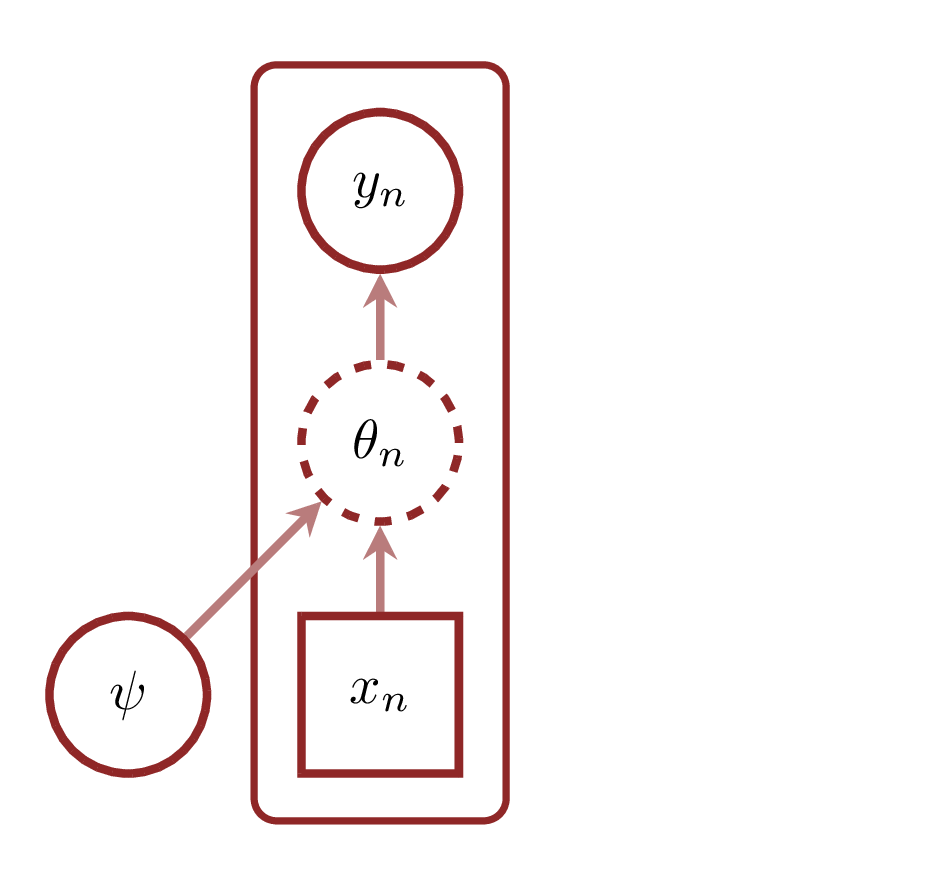
\includegraphics[width=0.5\textwidth,height=\textheight]{figures/2/2.png}

}

\caption{\label{fig-model2}One way to allow conversion outcomes to vary
with previous purchases is to replace the conversion probability
parameter with the output of a deterministic function of the previous
purchases.}

\end{figure}%

The model is not complete, however, until we have an explicit form for
this probability function. Specifically we need to engineer functional
behavior that is consistent with our domain expertise.

For example let's say that we believe that the conversion probability
should initially rise with previous purchases but also that any rise
cannot continue forever. In other words any rise should slow and
eventually saturate for sufficiently large previous purchases. One way
to accommodate this behavior is with the functional model \[
\theta(x, \psi)
= \theta(x, \psi_{1}, \psi_{2})
= \psi_{1} \cdot \left( 1 - \exp(- \psi_{2} \cdot x) \right).
\]

\begin{Shaded}
\begin{Highlighting}[]
\NormalTok{theta }\OtherTok{\textless{}{-}} \ControlFlowTok{function}\NormalTok{(x, psi1, psi2) \{}
\NormalTok{  psi1 }\SpecialCharTok{*}\NormalTok{ (}\SpecialCharTok{{-}}\FunctionTok{expm1}\NormalTok{(}\SpecialCharTok{{-}}\NormalTok{psi2 }\SpecialCharTok{*}\NormalTok{ x))}
\NormalTok{\}}
\end{Highlighting}
\end{Shaded}

Notice that as \(\psi_{2}\) goes to infinity the function
\(\theta(x, \psi_{1}, \psi_{2})\) converges to a constant function and
our model reduces to the previous model with \(\psi_{1}\) replacing
\(\theta\). In other words with this functional form our model
\emph{expands} upon the previous model by adding new functionality
\emph{but not excluding any existing functionality}. This helps make our
iterative model development robust to potential problems like
over-fitting.

At this point we need to develop a prior model for \(\psi_{1}\) and
\(\psi_{2}\) that ensures reasonable functional behaviors. Here we will
assume an independent component prior model, \[
\pi( \psi_{1}, \psi_{1}) = \pi(\psi_{1}) \, \pi(\psi_{2}).
\]

Because \(\psi_{1}\) determines the range of possible conversion
probabilities we can carry over the domain expertise that we elicited
about the aggregate conversion probability as a conservative prior model
for \(\psi_{1}\), \[
\pi( \psi_{1} ) = \mathrm{beta}( \psi_{1} \mid 0.5, 5.0).
\]

An appropriate prior model for \(\psi_{2}\) depends on what we know
about how quickly the conversion probability can saturate. In particular
the previous purchases where the conversion probability reaches half of
its maximum is given by \begin{align*}
\psi_{1} \, \frac{1}{2}
&=
\psi_{1} \,
\left( 1 - \exp \left( - \psi_{2} \cdot x_{\frac{1}{2}} \right) \right)
\\
\frac{1}{2}
&=
1 - \exp \left(- \psi_{2} \cdot x_{\frac{1}{2}} \right)
\\
\exp \left(- \psi_{2} \cdot x_{\frac{1}{2}} \right)
&=
\frac{1}{2}
\\
- \psi_{2} \cdot x_{\frac{1}{2}}
&=
\log \frac{1}{2}
\\
\psi_{2}
&=
\frac{\log 2}{x_{\frac{1}{2}}}.
\end{align*} Now let's say that we are fairly confident that it will
take at least \(2000\) USD of previous purchases to achieve reach five
times \(x_{\frac{1}{2}}\), \begin{align*}
5 \, x_{\frac{1}{2}} &> 2000 \, \mathrm{USD}
\\
x_{\frac{1}{2}} &> 400 \, \mathrm{USD}.
\end{align*} This implies that \begin{align*}
\psi_{2}
&=
\frac{\log 2}{x_{\frac{1}{2}}}
\\
&<
\frac{\log 2}{400} \, \mathrm{USD}^{-1}
\\
&<
1.7 \cdot 10^{-3} \, \mathrm{USD}^{-1}
\\
&\lessapprox 2 \, \mathrm{kUSD}^{-1}.
\end{align*} We can ensure this containment with a half-normal prior
model for \(\psi_{2}\), \[
\pi( \psi_{2} )
=
\text{half-normal} \left( \psi_{2} \mid 0, \frac{2}{2.57} \right).
\] For an explanation of the factor of \(2.57\) see Section 3.3 of my
\href{https://betanalpha.github.io/assets/case_studies/prior_modeling.html}{prior
modeling chapter}.

In developing this prior model we have considered the two parameters
\(\psi_{1}\) and \(\psi_{2}\) separately from each other even though
they interact when evaluating the conversion probability at a given
value for previous purchases. To verify that there are not any undesired
behaviors hiding in those interactions we can perform a prior
pushforward check where we visualize an ensemble of possible conversion
function behaviors. Fortunately none of these derived behaviors exhibit
any pathological behavior.

\begin{Shaded}
\begin{Highlighting}[]
\NormalTok{J }\OtherTok{\textless{}{-}} \DecValTok{50}
\NormalTok{nom\_colors }\OtherTok{\textless{}{-}} \FunctionTok{c}\NormalTok{(}\StringTok{"\#DCBCBC"}\NormalTok{, }\StringTok{"\#C79999"}\NormalTok{, }\StringTok{"\#B97C7C"}\NormalTok{,}
                \StringTok{"\#A25050"}\NormalTok{, }\StringTok{"\#8F2727"}\NormalTok{, }\StringTok{"\#7C0000"}\NormalTok{)}
\NormalTok{line\_colors }\OtherTok{\textless{}{-}} \FunctionTok{colormap}\NormalTok{(}\AttributeTok{colormap=}\NormalTok{nom\_colors, }\AttributeTok{nshades=}\NormalTok{J)}

\FunctionTok{par}\NormalTok{(}\AttributeTok{mfrow=}\FunctionTok{c}\NormalTok{(}\DecValTok{1}\NormalTok{, }\DecValTok{1}\NormalTok{), }\AttributeTok{mar=}\FunctionTok{c}\NormalTok{(}\DecValTok{5}\NormalTok{, }\DecValTok{5}\NormalTok{, }\DecValTok{3}\NormalTok{, }\DecValTok{1}\NormalTok{))}

\FunctionTok{plot}\NormalTok{(}\DecValTok{0}\NormalTok{, }\AttributeTok{type=}\StringTok{\textquotesingle{}n\textquotesingle{}}\NormalTok{,}
     \AttributeTok{xlim=}\FunctionTok{c}\NormalTok{(}\DecValTok{0}\NormalTok{, }\DecValTok{5000}\NormalTok{), }\AttributeTok{xlab=}\StringTok{"USD"}\NormalTok{,}
     \AttributeTok{ylim=}\FunctionTok{c}\NormalTok{(}\DecValTok{0}\NormalTok{, }\DecValTok{1}\NormalTok{), }\AttributeTok{ylab=}\StringTok{"Conversion Probability"}\NormalTok{)}

\ControlFlowTok{for}\NormalTok{ (j }\ControlFlowTok{in} \DecValTok{1}\SpecialCharTok{:}\NormalTok{J) \{}
\NormalTok{  psi1 }\OtherTok{\textless{}{-}} \FunctionTok{rbeta}\NormalTok{(}\DecValTok{1}\NormalTok{, }\FloatTok{0.5}\NormalTok{, }\DecValTok{5}\NormalTok{)}
\NormalTok{  psi2 }\OtherTok{\textless{}{-}} \FunctionTok{abs}\NormalTok{(}\FunctionTok{rnorm}\NormalTok{(}\DecValTok{1}\NormalTok{, }\DecValTok{0}\NormalTok{, }\DecValTok{2} \SpecialCharTok{/} \FloatTok{2.57}\NormalTok{))}
\NormalTok{  xs }\OtherTok{\textless{}{-}} \FunctionTok{seq}\NormalTok{(}\DecValTok{0}\NormalTok{, }\DecValTok{5000}\NormalTok{, }\DecValTok{10}\NormalTok{)}
\NormalTok{  ys }\OtherTok{\textless{}{-}} \FunctionTok{sapply}\NormalTok{(xs, }\ControlFlowTok{function}\NormalTok{(x) }\FunctionTok{theta}\NormalTok{(x, psi1, }\FloatTok{1e{-}3} \SpecialCharTok{*}\NormalTok{ psi2))}
  \FunctionTok{lines}\NormalTok{(xs, ys, }\AttributeTok{lwd=}\DecValTok{2}\NormalTok{, }\AttributeTok{col=}\NormalTok{line\_colors[j])}
\NormalTok{\}}
\end{Highlighting}
\end{Shaded}

\includegraphics{customer_conversion_files/figure-pdf/unnamed-chunk-19-1.pdf}

Armed with a carefully considered prior model we can let loose our
expanded model onto the observed data.

\begin{codelisting}

\caption{\texttt{model2.stan}}

\begin{Shaded}
\begin{Highlighting}[]
\KeywordTok{functions}\NormalTok{ \{}
  \CommentTok{// Saturating conversion probability function}
  \DataTypeTok{real}\NormalTok{ theta(}\DataTypeTok{real}\NormalTok{ x, }\DataTypeTok{real}\NormalTok{ psi1, }\DataTypeTok{real}\NormalTok{ psi2) \{}
    \ControlFlowTok{return}\NormalTok{ psi1 * ({-}expm1({-}psi2 * x));}
\NormalTok{  \}}
\NormalTok{\}}

\KeywordTok{data}\NormalTok{ \{}
  \CommentTok{// Observed data}
  \DataTypeTok{int}\NormalTok{\textless{}}\KeywordTok{lower}\NormalTok{=}\DecValTok{1}\NormalTok{\textgreater{} N;                    }\CommentTok{// Number of unique visits}
  \DataTypeTok{array}\NormalTok{[N] }\DataTypeTok{int}\NormalTok{\textless{}}\KeywordTok{lower}\NormalTok{=}\DecValTok{0}\NormalTok{, }\KeywordTok{upper}\NormalTok{=}\DecValTok{1}\NormalTok{\textgreater{} y;  }\CommentTok{// Conversion indicator}
  \DataTypeTok{array}\NormalTok{[N] }\DataTypeTok{real}\NormalTok{ x;                   }\CommentTok{// Previous purchases (USD)}
\NormalTok{\}}

\KeywordTok{parameters}\NormalTok{ \{}
  \DataTypeTok{real}\NormalTok{\textless{}}\KeywordTok{lower}\NormalTok{=}\DecValTok{0}\NormalTok{, }\KeywordTok{upper}\NormalTok{=}\DecValTok{1}\NormalTok{\textgreater{} psi1; }\CommentTok{// Maximum conversion probability}
  \DataTypeTok{real}\NormalTok{\textless{}}\KeywordTok{lower}\NormalTok{=}\DecValTok{0}\NormalTok{\textgreater{} psi2;          }\CommentTok{// Rate of saturation (1 / kUSD)}
\NormalTok{\}}

\KeywordTok{model}\NormalTok{ \{}
  \CommentTok{// Prior model}
\NormalTok{  psi1 \textasciitilde{} beta(}\FloatTok{0.5}\NormalTok{, }\FloatTok{5.0}\NormalTok{);        }\CommentTok{// 0 \textless{}\textasciitilde{} psi1 \textless{}\textasciitilde{} 0.5}
\NormalTok{  psi2 \textasciitilde{} normal(}\DecValTok{0}\NormalTok{, }\FloatTok{2.0}\NormalTok{ / }\FloatTok{2.57}\NormalTok{); }\CommentTok{// 0 \textless{}\textasciitilde{} psi2 \textless{}\textasciitilde{} 2}

  \CommentTok{// Observational model}
  \ControlFlowTok{for}\NormalTok{ (n }\ControlFlowTok{in} \DecValTok{1}\NormalTok{:N) \{}
    \KeywordTok{target +=}\NormalTok{ bernoulli\_lpmf(y[n] | theta(x[n], psi1, }\FloatTok{1e{-}3}\NormalTok{ * psi2));}
\NormalTok{  \}}
\NormalTok{\}}

\KeywordTok{generated quantities}\NormalTok{ \{}
  \CommentTok{// Posterior predictions}
  \DataTypeTok{array}\NormalTok{[N] }\DataTypeTok{real}\NormalTok{ y\_pred;}
  \DataTypeTok{real}\NormalTok{ p\_hat\_pred;}

  \ControlFlowTok{for}\NormalTok{ (n }\ControlFlowTok{in} \DecValTok{1}\NormalTok{:N) \{}
\NormalTok{    y\_pred[n] = bernoulli\_rng(theta(x[n], psi1, }\FloatTok{1e{-}3}\NormalTok{ * psi2));}
\NormalTok{  \}}
\NormalTok{  p\_hat\_pred = mean(y\_pred);}
\NormalTok{\}}
\end{Highlighting}
\end{Shaded}

\end{codelisting}

\begin{Shaded}
\begin{Highlighting}[]
\NormalTok{fit }\OtherTok{\textless{}{-}} \FunctionTok{stan}\NormalTok{(}\AttributeTok{file=}\StringTok{"stan\_programs/model2.stan"}\NormalTok{,}
            \AttributeTok{data=}\NormalTok{data, }\AttributeTok{seed=}\DecValTok{8438338}\NormalTok{,}
            \AttributeTok{warmup=}\DecValTok{1000}\NormalTok{, }\AttributeTok{iter=}\DecValTok{2024}\NormalTok{, }\AttributeTok{refresh=}\DecValTok{0}\NormalTok{)}
\end{Highlighting}
\end{Shaded}

Fortunately the computational diagnostics are clean.

\begin{Shaded}
\begin{Highlighting}[]
\NormalTok{diagnostics2 }\OtherTok{\textless{}{-}}\NormalTok{ util}\SpecialCharTok{$}\FunctionTok{extract\_hmc\_diagnostics}\NormalTok{(fit)}
\NormalTok{util}\SpecialCharTok{$}\FunctionTok{check\_all\_hmc\_diagnostics}\NormalTok{(diagnostics2)}
\end{Highlighting}
\end{Shaded}

\begin{verbatim}
  All Hamiltonian Monte Carlo diagnostics are consistent with reliable
Markov chain Monte Carlo.
\end{verbatim}

\begin{Shaded}
\begin{Highlighting}[]
\NormalTok{samples2 }\OtherTok{\textless{}{-}}\NormalTok{ util}\SpecialCharTok{$}\FunctionTok{extract\_expectands}\NormalTok{(fit)}
\NormalTok{base\_samples }\OtherTok{\textless{}{-}}\NormalTok{ util}\SpecialCharTok{$}\FunctionTok{filter\_expectands}\NormalTok{(samples2,}
                                       \FunctionTok{c}\NormalTok{(}\StringTok{\textquotesingle{}psi1\textquotesingle{}}\NormalTok{, }\StringTok{\textquotesingle{}psi2\textquotesingle{}}\NormalTok{))}
\NormalTok{util}\SpecialCharTok{$}\FunctionTok{check\_all\_expectand\_diagnostics}\NormalTok{(base\_samples)}
\end{Highlighting}
\end{Shaded}

\begin{verbatim}
All expectands checked appear to be behaving well enough for reliable
Markov chain Monte Carlo estimation.
\end{verbatim}

The retrodictive behavior in the empirical frequency summary statistic
also looks good.

\begin{Shaded}
\begin{Highlighting}[]
\FunctionTok{par}\NormalTok{(}\AttributeTok{mfrow=}\FunctionTok{c}\NormalTok{(}\DecValTok{1}\NormalTok{, }\DecValTok{1}\NormalTok{), }\AttributeTok{mar=}\FunctionTok{c}\NormalTok{(}\DecValTok{5}\NormalTok{, }\DecValTok{5}\NormalTok{, }\DecValTok{3}\NormalTok{, }\DecValTok{1}\NormalTok{))}

\NormalTok{util}\SpecialCharTok{$}\FunctionTok{plot\_expectand\_pushforward}\NormalTok{(samples2[[}\StringTok{\textquotesingle{}p\_hat\_pred\textquotesingle{}}\NormalTok{]], }\DecValTok{20}\NormalTok{,}
                                \AttributeTok{display\_name=}\StringTok{"Aggregate Conversion Frequency"}\NormalTok{,}
                                \AttributeTok{baseline=}\FunctionTok{mean}\NormalTok{(data}\SpecialCharTok{$}\NormalTok{y))}
\end{Highlighting}
\end{Shaded}

\includegraphics{customer_conversion_files/figure-pdf/unnamed-chunk-22-1.pdf}

While the retrodictive behavior in the binned empirical frequencies is a
substantial improvement to that of the previous model it still leaves
much to be desired. In particular the posterior predictive behavior
starts at zero conversion frequency whereas the observed conversion
frequencies appear to start at a non-zero value.

\begin{Shaded}
\begin{Highlighting}[]
\FunctionTok{par}\NormalTok{(}\AttributeTok{mfrow=}\FunctionTok{c}\NormalTok{(}\DecValTok{1}\NormalTok{, }\DecValTok{1}\NormalTok{), }\AttributeTok{mar=}\FunctionTok{c}\NormalTok{(}\DecValTok{5}\NormalTok{, }\DecValTok{5}\NormalTok{, }\DecValTok{3}\NormalTok{, }\DecValTok{1}\NormalTok{))}

\NormalTok{pred\_names }\OtherTok{\textless{}{-}} \FunctionTok{sapply}\NormalTok{(}\DecValTok{1}\SpecialCharTok{:}\NormalTok{data}\SpecialCharTok{$}\NormalTok{N, }\ControlFlowTok{function}\NormalTok{(n) }\FunctionTok{paste0}\NormalTok{(}\StringTok{\textquotesingle{}y\_pred[\textquotesingle{}}\NormalTok{, n, }\StringTok{\textquotesingle{}]\textquotesingle{}}\NormalTok{))}
\NormalTok{util}\SpecialCharTok{$}\FunctionTok{plot\_conditional\_mean\_quantiles}\NormalTok{(samples2, pred\_names, data}\SpecialCharTok{$}\NormalTok{x,}
                                     \DecValTok{0}\NormalTok{, }\DecValTok{6120}\NormalTok{, }\DecValTok{153}\NormalTok{,}
                                     \AttributeTok{baseline\_values=}\NormalTok{data}\SpecialCharTok{$}\NormalTok{y,}
                                     \AttributeTok{xlab=}\StringTok{"Previous Purchases (USD)"}\NormalTok{,}
                                     \AttributeTok{ylab=}\StringTok{"Binned Conversion Frequency"}\NormalTok{)}
\end{Highlighting}
\end{Shaded}

\includegraphics{customer_conversion_files/figure-pdf/unnamed-chunk-23-1.pdf}

We can focus on these discrepancies by zooming into smaller previous
purchases.

\begin{Shaded}
\begin{Highlighting}[]
\FunctionTok{par}\NormalTok{(}\AttributeTok{mfrow=}\FunctionTok{c}\NormalTok{(}\DecValTok{1}\NormalTok{, }\DecValTok{1}\NormalTok{), }\AttributeTok{mar=}\FunctionTok{c}\NormalTok{(}\DecValTok{5}\NormalTok{, }\DecValTok{5}\NormalTok{, }\DecValTok{3}\NormalTok{, }\DecValTok{1}\NormalTok{))}

\NormalTok{pred\_names }\OtherTok{\textless{}{-}} \FunctionTok{sapply}\NormalTok{(}\DecValTok{1}\SpecialCharTok{:}\NormalTok{data}\SpecialCharTok{$}\NormalTok{N, }\ControlFlowTok{function}\NormalTok{(n) }\FunctionTok{paste0}\NormalTok{(}\StringTok{\textquotesingle{}y\_pred[\textquotesingle{}}\NormalTok{, n, }\StringTok{\textquotesingle{}]\textquotesingle{}}\NormalTok{))}
\NormalTok{util}\SpecialCharTok{$}\FunctionTok{plot\_conditional\_mean\_quantiles}\NormalTok{(samples2, pred\_names, data}\SpecialCharTok{$}\NormalTok{x,}
                                     \DecValTok{0}\NormalTok{, }\DecValTok{1000}\NormalTok{, }\DecValTok{50}\NormalTok{,}
                                     \AttributeTok{baseline\_values=}\NormalTok{data}\SpecialCharTok{$}\NormalTok{y,}
                                     \AttributeTok{xlab=}\StringTok{"Previous Purchases (USD)"}\NormalTok{,}
                                     \AttributeTok{ylab=}\StringTok{"Binned Conversion Frequency"}\NormalTok{)}
\end{Highlighting}
\end{Shaded}

\begin{verbatim}
Warning in check_bin_containment(bin_min, bin_max, obs_xs, "conditioning
value"): 809 conditioning values (53.9%) fell above the binning.
\end{verbatim}

\includegraphics{customer_conversion_files/figure-pdf/unnamed-chunk-24-1.pdf}

The challenge now is to leverage our domain expertise into a hypothesize
about what could be inadequate about our current modeling assumptions.
Why might new customers with no previous purchases exhibit a non-zero
conversion probability?

\subsection{Model 3}\label{model-3}

One of the subtle issues with domain expertise is that it takes energy
and time to transform from implicit, qualitative information to
explicit, quantitative information. After a finite amount of effort we
will only ever be working with a finite amount of our, or our team's,
domain expertise. The challenge to making elicitation productive is
identifying what kind of domain expertise to elicit. Conveniently
modeling problems are often highly effective at triggering unused
knowledge.

For example in trying to reason about non-zero initial conversion
probabilities we might remember, be informed by our collaborators, or
even learn from public literature that our target market is not
homogeneous but instead consists of typical customers and another, more
engaged group of special customers. This might happen, for instance,
when the engagement we are offering is branded with a popular cultural
icon, such as a sports team or celebrity, and fans of that icon will
have the same propensity to engage regardless of their previous
business.

This narrative suggests not one but rather two observational models: \[
\text{Bernoulli} \,(y_{n} \mid \theta \, (x_{n}, \psi))
\] for the regular customers and \[
\text{Bernoulli} \,(y_{n} \mid \theta^{\text{VIP}})
\] for the very important customers, or \emph{VIPs}.

The problem, however, is that we don't know to which of these groups a
given customer in our observed data belongs, and hence which data
generating process to apply. In order to account for the possibility
that each customer could belong to either group we can appeal to a
mixture model with the mixture parameter \(\lambda\) determining the
overall proportion of VIP customers (Figure~\ref{fig-model3}),
\begin{align*}
\pi(y_{1}, \ldots, y_{N}, &\psi, \theta^{\text{VIP}}, \lambda;
    x_{1}, \ldots, x_{N})
\\
=& \;\;
\left[
\prod_{n = 1}^{N}
  (1 - \lambda) \cdot \text{Bernoulli} \,(y_{n} \mid \theta \, (x_{n}, \psi))
+ \lambda \cdot \text{Bernoulli} \,(y_{n} \mid \theta^{\text{VIP}})
\right]
\\
& \cdot
\pi(\psi) \, \pi(\theta^{\text{VIP}}) \, \pi(\lambda).
\end{align*}

\begin{figure}

\centering{

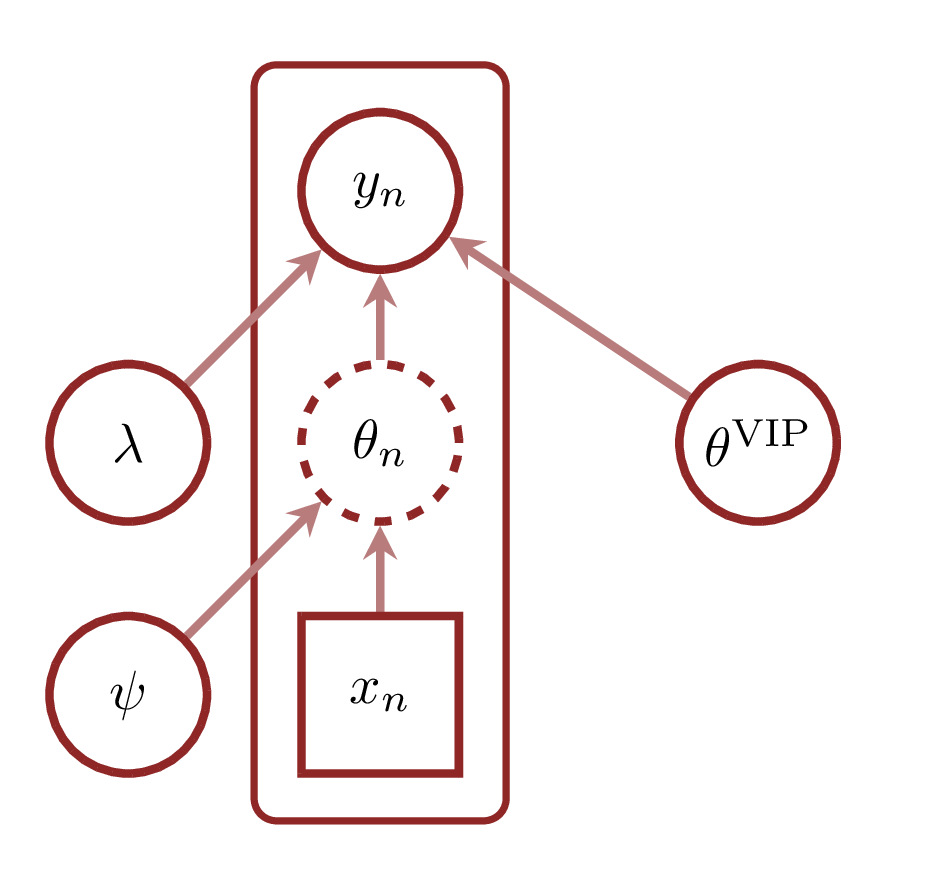
\includegraphics[width=0.5\textwidth,height=\textheight]{figures/3/3.png}

}

\caption{\label{fig-model3}A mixture model allows us to integrate two
distinct data generating processes together even when we don't know from
which data generating process a given observation was drawn.}

\end{figure}%

All that remains is a prior model for the proportion of VIP customers
\(\lambda\) and the conversion probability of the VIP customers
\(\theta^{\text{VIP}}\). As always these prior models depend on our
domain expertise, which in this case is entirely hypothetical. For
example if are aware of an ongoing promotion that is likely to resonate
with the VIP customers then we might engineer a prior model that
concentrates on large values of \(\theta^{\text{VIP}}\). Here we'll take
a diffuse prior model for \(\lambda\), \[
\pi(\lambda) = \mathrm{beta}(\lambda \mid 1, 1),
\] and a prior model that contains \(\theta^{\text{VIP}}\) above \(0.5\)
to account for the higher engagement, \[
\pi(\theta^{\text{VIP}}) = \mathrm{beta}(\theta^{\text{VIP}} \mid 5.0, 0.5).
\]

Let's implement this further expanded model in \texttt{Stan} and then
take it for a spin.

\begin{codelisting}

\caption{\texttt{model3.stan}}

\begin{Shaded}
\begin{Highlighting}[]
\KeywordTok{functions}\NormalTok{ \{}
  \CommentTok{// Saturating conversion probability function}
  \DataTypeTok{real}\NormalTok{ theta(}\DataTypeTok{real}\NormalTok{ x, }\DataTypeTok{real}\NormalTok{ psi1, }\DataTypeTok{real}\NormalTok{ psi2) \{}
    \ControlFlowTok{return}\NormalTok{ psi1 * ({-}expm1({-}psi2 * x));}
\NormalTok{  \}}
\NormalTok{\}}

\KeywordTok{data}\NormalTok{ \{}
  \CommentTok{// Observed data}
  \DataTypeTok{int}\NormalTok{\textless{}}\KeywordTok{lower}\NormalTok{=}\DecValTok{1}\NormalTok{\textgreater{} N;                    }\CommentTok{// Number of unique visits}
  \DataTypeTok{array}\NormalTok{[N] }\DataTypeTok{int}\NormalTok{\textless{}}\KeywordTok{lower}\NormalTok{=}\DecValTok{0}\NormalTok{, }\KeywordTok{upper}\NormalTok{=}\DecValTok{1}\NormalTok{\textgreater{} y;  }\CommentTok{// Conversion indicator}
  \DataTypeTok{array}\NormalTok{[N] }\DataTypeTok{real}\NormalTok{ x;                   }\CommentTok{// Previous purchases (USD)}
\NormalTok{\}}

\KeywordTok{parameters}\NormalTok{ \{}
  \DataTypeTok{real}\NormalTok{\textless{}}\KeywordTok{lower}\NormalTok{=}\DecValTok{0}\NormalTok{, }\KeywordTok{upper}\NormalTok{=}\DecValTok{1}\NormalTok{\textgreater{} psi1;      }\CommentTok{// Maximum conversion probability}
  \DataTypeTok{real}\NormalTok{\textless{}}\KeywordTok{lower}\NormalTok{=}\DecValTok{0}\NormalTok{\textgreater{} psi2;               }\CommentTok{// Rate of saturation (1 / kUSD)}
  \DataTypeTok{real}\NormalTok{\textless{}}\KeywordTok{lower}\NormalTok{=}\DecValTok{0}\NormalTok{, }\KeywordTok{upper}\NormalTok{=}\DecValTok{1}\NormalTok{\textgreater{} lambda;    }\CommentTok{// Proportion of VIP visitors}
  \DataTypeTok{real}\NormalTok{\textless{}}\KeywordTok{lower}\NormalTok{=}\DecValTok{0}\NormalTok{, }\KeywordTok{upper}\NormalTok{=}\DecValTok{1}\NormalTok{\textgreater{} theta\_VIP; }\CommentTok{// VIP conversion probability}
\NormalTok{\}}

\KeywordTok{model}\NormalTok{ \{}
  \CommentTok{// Prior model}
\NormalTok{  psi1 \textasciitilde{} beta(}\FloatTok{0.5}\NormalTok{, }\FloatTok{5.0}\NormalTok{);        }\CommentTok{// 0   \textless{}\textasciitilde{}    psi1   \textless{}\textasciitilde{} 0.5}
\NormalTok{  psi2 \textasciitilde{} normal(}\DecValTok{0}\NormalTok{, }\FloatTok{2.0}\NormalTok{ / }\FloatTok{2.57}\NormalTok{); }\CommentTok{// 0   \textless{}\textasciitilde{}    psi2   \textless{}\textasciitilde{} 2}
\NormalTok{  lambda \textasciitilde{} beta(}\DecValTok{1}\NormalTok{, }\DecValTok{1}\NormalTok{);          }\CommentTok{// Uniform probability density function}
\NormalTok{  theta\_VIP \textasciitilde{} beta(}\FloatTok{5.0}\NormalTok{, }\FloatTok{0.5}\NormalTok{);   }\CommentTok{// 0.5 \textless{}\textasciitilde{} theta\_VIP \textless{}\textasciitilde{} 1}

  \CommentTok{// Observational model}
  \ControlFlowTok{for}\NormalTok{ (n }\ControlFlowTok{in} \DecValTok{1}\NormalTok{:N) \{}
    \KeywordTok{target +=}\NormalTok{ log\_mix(lambda,}
\NormalTok{                      bernoulli\_lpmf(y[n] | theta\_VIP),}
\NormalTok{                      bernoulli\_lpmf(y[n] | theta(x[n], psi1, }\FloatTok{1e{-}3}\NormalTok{ * psi2)));}
\NormalTok{  \}}
\NormalTok{\}}

\KeywordTok{generated quantities}\NormalTok{ \{}
  \CommentTok{// Posterior predictions}
  \DataTypeTok{array}\NormalTok{[N] }\DataTypeTok{real}\NormalTok{ y\_pred;}
  \DataTypeTok{real}\NormalTok{ p\_hat\_pred;}

  \ControlFlowTok{for}\NormalTok{ (n }\ControlFlowTok{in} \DecValTok{1}\NormalTok{:N) \{}
    \ControlFlowTok{if}\NormalTok{ (bernoulli\_rng(lambda)) \{}
\NormalTok{      y\_pred[n] = bernoulli\_rng(theta\_VIP);}
\NormalTok{    \} }\ControlFlowTok{else}\NormalTok{ \{}
\NormalTok{      y\_pred[n] = bernoulli\_rng(theta(x[n], psi1, }\FloatTok{1e{-}3}\NormalTok{ * psi2));}
\NormalTok{    \}}
\NormalTok{  \}}
\NormalTok{  p\_hat\_pred = mean(y\_pred);}
\NormalTok{\}}
\end{Highlighting}
\end{Shaded}

\end{codelisting}

\begin{Shaded}
\begin{Highlighting}[]
\NormalTok{fit }\OtherTok{\textless{}{-}} \FunctionTok{stan}\NormalTok{(}\AttributeTok{file=}\StringTok{"stan\_programs/model3.stan"}\NormalTok{,}
            \AttributeTok{data=}\NormalTok{data, }\AttributeTok{seed=}\DecValTok{8438338}\NormalTok{,}
            \AttributeTok{warmup=}\DecValTok{1000}\NormalTok{, }\AttributeTok{iter=}\DecValTok{2024}\NormalTok{, }\AttributeTok{refresh=}\DecValTok{0}\NormalTok{)}
\end{Highlighting}
\end{Shaded}

Unfortunately the computational diagnostics are no longer as quiet as
they have been. The divergent transitions indicate that there are model
configurations consistent with the data that \texttt{Stan} has not been
able to explore. For more on dealing with divergences see my chapter on
\href{https://betanalpha.github.io/assets/case_studies/identifiability.html}{inferential
degeneracy}.

\begin{Shaded}
\begin{Highlighting}[]
\NormalTok{diagnostics3 }\OtherTok{\textless{}{-}}\NormalTok{ util}\SpecialCharTok{$}\FunctionTok{extract\_hmc\_diagnostics}\NormalTok{(fit)}
\NormalTok{util}\SpecialCharTok{$}\FunctionTok{check\_all\_hmc\_diagnostics}\NormalTok{(diagnostics3)}
\end{Highlighting}
\end{Shaded}

\begin{verbatim}
  Chain 1: 2 of 1024 transitions (0.2%) diverged.

  Chain 2: 2 of 1024 transitions (0.2%) diverged.

  Chain 3: 8 of 1024 transitions (0.8%) diverged.

  Chain 4: 7 of 1024 transitions (0.7%) diverged.

  Divergent Hamiltonian transitions result from unstable numerical
trajectories.  These instabilities are often due to degenerate target
geometry, especially "pinches".  If there are only a small number of
divergences then running with adept_delta larger than 0.801 may reduce
the instabilities at the cost of more expensive Hamiltonian
transitions.
\end{verbatim}

\begin{Shaded}
\begin{Highlighting}[]
\NormalTok{samples3 }\OtherTok{\textless{}{-}}\NormalTok{ util}\SpecialCharTok{$}\FunctionTok{extract\_expectands}\NormalTok{(fit)}
\NormalTok{base\_samples }\OtherTok{\textless{}{-}}\NormalTok{ util}\SpecialCharTok{$}\FunctionTok{filter\_expectands}\NormalTok{(samples3,}
                                       \FunctionTok{c}\NormalTok{(}\StringTok{\textquotesingle{}psi1\textquotesingle{}}\NormalTok{, }\StringTok{\textquotesingle{}psi2\textquotesingle{}}\NormalTok{,}
                                         \StringTok{\textquotesingle{}lambda\textquotesingle{}}\NormalTok{, }\StringTok{\textquotesingle{}theta\_VIP\textquotesingle{}}\NormalTok{))}
\NormalTok{util}\SpecialCharTok{$}\FunctionTok{check\_all\_expectand\_diagnostics}\NormalTok{(base\_samples)}
\end{Highlighting}
\end{Shaded}

\begin{verbatim}
All expectands checked appear to be behaving well enough for reliable
Markov chain Monte Carlo estimation.
\end{verbatim}

One way that we can identify where problems might be arising in the
model configuration space is to examine pairs plots with the divergent
and non-divergent Markov chain iterations drawn in different colors. To
better assess the computational issues we'll first unconstrain each
parameter, mirroring how \texttt{Stan} automatically accommodates
parameter constraints.

\begin{Shaded}
\begin{Highlighting}[]
\NormalTok{names }\OtherTok{\textless{}{-}} \FunctionTok{c}\NormalTok{(}\StringTok{\textquotesingle{}psi1\textquotesingle{}}\NormalTok{, }\StringTok{\textquotesingle{}psi2\textquotesingle{}}\NormalTok{, }\StringTok{\textquotesingle{}lambda\textquotesingle{}}\NormalTok{, }\StringTok{\textquotesingle{}theta\_VIP\textquotesingle{}}\NormalTok{)}
\NormalTok{util}\SpecialCharTok{$}\FunctionTok{plot\_div\_pairs}\NormalTok{(names, names, samples3, diagnostics3,}
                    \AttributeTok{transforms=}\FunctionTok{list}\NormalTok{(}\StringTok{"psi1"} \OtherTok{=} \DecValTok{2}\NormalTok{, }\StringTok{"psi2"} \OtherTok{=} \DecValTok{1}\NormalTok{,}
                                    \StringTok{"lambda"} \OtherTok{=} \DecValTok{2}\NormalTok{, }\StringTok{"theta\_VIP"} \OtherTok{=} \DecValTok{2}\NormalTok{))}
\end{Highlighting}
\end{Shaded}

\includegraphics{customer_conversion_files/figure-pdf/unnamed-chunk-27-1.pdf}

We see that the divergent iterations seem to concentrate in a region of
the model configuration space where the posterior samples of
\(\mathrm{logit}(\lambda)\) and \(\mathrm{logit}(\theta^{\text{VIP}})\)
pinch together.

\begin{Shaded}
\begin{Highlighting}[]
\NormalTok{util}\SpecialCharTok{$}\FunctionTok{plot\_div\_pairs}\NormalTok{(}\FunctionTok{c}\NormalTok{(}\StringTok{\textquotesingle{}lambda\textquotesingle{}}\NormalTok{), }\FunctionTok{c}\NormalTok{(}\StringTok{\textquotesingle{}theta\_VIP\textquotesingle{}}\NormalTok{), samples3, diagnostics3,}
                    \AttributeTok{transforms=}\FunctionTok{list}\NormalTok{(}\StringTok{"lambda"} \OtherTok{=} \DecValTok{2}\NormalTok{, }\StringTok{"theta\_VIP"} \OtherTok{=} \DecValTok{2}\NormalTok{))}
\end{Highlighting}
\end{Shaded}

\includegraphics{customer_conversion_files/figure-pdf/unnamed-chunk-28-1.pdf}

The problem here is that our model is now sufficiently flexible that
many distinct behaviors are similarly consistent with the observed data.
In particular the observations appear to be insensitive to model
configurations with a larger proportion of VIP customers and smaller VIP
conversion probability and model configurations with a smaller
proportion of VIP customers and larger VIP conversion probabilities. The
posterior distribution extends out to all of these consistent model
configurations, but those uncertainties frustrate accurate computation.

One way to force a more refined, but more expensive, exploration with
the dynamic Hamiltonian Monte Carlo sampler in \texttt{Stan} is to force
a less aggressive step size adaptation. This is done by increasing the
\texttt{adapt\_delta} configuration from it's default value of \(0.8\).
Here we'll try \(0.99\).

\begin{Shaded}
\begin{Highlighting}[]
\NormalTok{fit }\OtherTok{\textless{}{-}} \FunctionTok{stan}\NormalTok{(}\AttributeTok{file=}\StringTok{"stan\_programs/model3.stan"}\NormalTok{,}
            \AttributeTok{data=}\NormalTok{data, }\AttributeTok{seed=}\DecValTok{8438338}\NormalTok{,}
            \AttributeTok{warmup=}\DecValTok{1000}\NormalTok{, }\AttributeTok{iter=}\DecValTok{2024}\NormalTok{, }\AttributeTok{refresh=}\DecValTok{0}\NormalTok{,}
            \AttributeTok{control=}\FunctionTok{list}\NormalTok{(}\StringTok{\textquotesingle{}adapt\_delta\textquotesingle{}}\OtherTok{=}\FloatTok{0.99}\NormalTok{))}
\end{Highlighting}
\end{Shaded}

It looks like this may have done the trick as we no longer see any
divergence warnings.

\begin{Shaded}
\begin{Highlighting}[]
\NormalTok{diagnostics3\_99 }\OtherTok{\textless{}{-}}\NormalTok{ util}\SpecialCharTok{$}\FunctionTok{extract\_hmc\_diagnostics}\NormalTok{(fit)}
\NormalTok{util}\SpecialCharTok{$}\FunctionTok{check\_all\_hmc\_diagnostics}\NormalTok{(diagnostics3\_99)}
\end{Highlighting}
\end{Shaded}

\begin{verbatim}
  All Hamiltonian Monte Carlo diagnostics are consistent with reliable
Markov chain Monte Carlo.
\end{verbatim}

\begin{Shaded}
\begin{Highlighting}[]
\NormalTok{samples3\_99 }\OtherTok{\textless{}{-}}\NormalTok{ util}\SpecialCharTok{$}\FunctionTok{extract\_expectands}\NormalTok{(fit)}
\NormalTok{base\_samples }\OtherTok{\textless{}{-}}\NormalTok{ util}\SpecialCharTok{$}\FunctionTok{filter\_expectands}\NormalTok{(samples3\_99,}
                                       \FunctionTok{c}\NormalTok{(}\StringTok{\textquotesingle{}psi1\textquotesingle{}}\NormalTok{, }\StringTok{\textquotesingle{}psi2\textquotesingle{}}\NormalTok{,}
                                         \StringTok{\textquotesingle{}lambda\textquotesingle{}}\NormalTok{, }\StringTok{\textquotesingle{}theta\_VIP\textquotesingle{}}\NormalTok{))}
\NormalTok{util}\SpecialCharTok{$}\FunctionTok{check\_all\_expectand\_diagnostics}\NormalTok{(base\_samples)}
\end{Highlighting}
\end{Shaded}

\begin{verbatim}
All expectands checked appear to be behaving well enough for reliable
Markov chain Monte Carlo estimation.
\end{verbatim}

Indeed comparing the two posterior quantifications we can see that using
a less aggressive adaptation allows us to capture more model behaviors
than before. These new model configurations have always been consistent
with the observed data, they were just ignored by our first, inaccurate
fit.

\begin{Shaded}
\begin{Highlighting}[]
\FunctionTok{par}\NormalTok{(}\AttributeTok{mfrow=}\FunctionTok{c}\NormalTok{(}\DecValTok{1}\NormalTok{, }\DecValTok{1}\NormalTok{))}

\NormalTok{logit }\OtherTok{\textless{}{-}} \ControlFlowTok{function}\NormalTok{(ps) \{}
  \FunctionTok{log}\NormalTok{(ps }\SpecialCharTok{/}\NormalTok{ (}\DecValTok{1} \SpecialCharTok{{-}}\NormalTok{ ps))}
\NormalTok{\}}

\FunctionTok{plot}\NormalTok{(}\FunctionTok{logit}\NormalTok{(}\FunctionTok{c}\NormalTok{(samples3\_99[}\StringTok{\textquotesingle{}lambda\textquotesingle{}}\NormalTok{], }\AttributeTok{recursive=}\ConstantTok{TRUE}\NormalTok{)),}
     \FunctionTok{logit}\NormalTok{(}\FunctionTok{c}\NormalTok{(samples3\_99[}\StringTok{\textquotesingle{}theta\_VIP\textquotesingle{}}\NormalTok{], }\AttributeTok{recursive=}\ConstantTok{TRUE}\NormalTok{)),}
     \AttributeTok{col=}\NormalTok{util}\SpecialCharTok{$}\NormalTok{c\_dark, }\AttributeTok{pch=}\DecValTok{16}\NormalTok{, }\AttributeTok{cex=}\FloatTok{0.8}\NormalTok{,}
     \AttributeTok{xlab=}\StringTok{"logit(lambda)"}\NormalTok{, }\AttributeTok{ylab=}\StringTok{"logit(theta\_VIP)"}\NormalTok{)}

\FunctionTok{points}\NormalTok{(}\FunctionTok{logit}\NormalTok{(}\FunctionTok{c}\NormalTok{(samples3[}\StringTok{\textquotesingle{}lambda\textquotesingle{}}\NormalTok{], }\AttributeTok{recursive=}\ConstantTok{TRUE}\NormalTok{)),}
       \FunctionTok{logit}\NormalTok{(}\FunctionTok{c}\NormalTok{(samples3[}\StringTok{\textquotesingle{}theta\_VIP\textquotesingle{}}\NormalTok{], }\AttributeTok{recursive=}\ConstantTok{TRUE}\NormalTok{)),}
       \AttributeTok{col=}\NormalTok{util}\SpecialCharTok{$}\NormalTok{c\_light, }\AttributeTok{pch=}\DecValTok{16}\NormalTok{, }\AttributeTok{cex=}\FloatTok{0.8}\NormalTok{)}
\end{Highlighting}
\end{Shaded}

\includegraphics{customer_conversion_files/figure-pdf/unnamed-chunk-31-1.pdf}

With an accurate posterior quantification we can consider the
retrodictive performance of this model. The aggregate conversion
frequency continues to show no signs of retrodictive tension.

\begin{Shaded}
\begin{Highlighting}[]
\FunctionTok{par}\NormalTok{(}\AttributeTok{mfrow=}\FunctionTok{c}\NormalTok{(}\DecValTok{1}\NormalTok{, }\DecValTok{1}\NormalTok{), }\AttributeTok{mar=}\FunctionTok{c}\NormalTok{(}\DecValTok{5}\NormalTok{, }\DecValTok{5}\NormalTok{, }\DecValTok{3}\NormalTok{, }\DecValTok{1}\NormalTok{))}

\NormalTok{util}\SpecialCharTok{$}\FunctionTok{plot\_expectand\_pushforward}\NormalTok{(samples3\_99[[}\StringTok{\textquotesingle{}p\_hat\_pred\textquotesingle{}}\NormalTok{]], }\DecValTok{20}\NormalTok{,}
                                \AttributeTok{display\_name=}\StringTok{"Aggregate Conversion Frequency"}\NormalTok{,}
                                \AttributeTok{baseline=}\FunctionTok{mean}\NormalTok{(data}\SpecialCharTok{$}\NormalTok{y))}
\end{Highlighting}
\end{Shaded}

\includegraphics{customer_conversion_files/figure-pdf/unnamed-chunk-32-1.pdf}

Now, however, the retrodictive behavior for the binned conversion
frequencies is much better. Allowing for two groups of customers has
finally allowed our model to adequately recover the behavior of the
observed data.

\begin{Shaded}
\begin{Highlighting}[]
\FunctionTok{par}\NormalTok{(}\AttributeTok{mfrow=}\FunctionTok{c}\NormalTok{(}\DecValTok{1}\NormalTok{, }\DecValTok{1}\NormalTok{), }\AttributeTok{mar=}\FunctionTok{c}\NormalTok{(}\DecValTok{5}\NormalTok{, }\DecValTok{5}\NormalTok{, }\DecValTok{3}\NormalTok{, }\DecValTok{1}\NormalTok{))}

\NormalTok{pred\_names }\OtherTok{\textless{}{-}} \FunctionTok{sapply}\NormalTok{(}\DecValTok{1}\SpecialCharTok{:}\NormalTok{data}\SpecialCharTok{$}\NormalTok{N, }\ControlFlowTok{function}\NormalTok{(n) }\FunctionTok{paste0}\NormalTok{(}\StringTok{\textquotesingle{}y\_pred[\textquotesingle{}}\NormalTok{, n, }\StringTok{\textquotesingle{}]\textquotesingle{}}\NormalTok{))}
\NormalTok{util}\SpecialCharTok{$}\FunctionTok{plot\_conditional\_mean\_quantiles}\NormalTok{(samples3\_99, pred\_names, data}\SpecialCharTok{$}\NormalTok{x,}
                                     \DecValTok{0}\NormalTok{, }\DecValTok{6120}\NormalTok{, }\DecValTok{153}\NormalTok{,}
                                     \AttributeTok{baseline\_values=}\NormalTok{data}\SpecialCharTok{$}\NormalTok{y,}
                                     \AttributeTok{xlab=}\StringTok{"Previous Purchases (USD)"}\NormalTok{,}
                                     \AttributeTok{ylab=}\StringTok{"Binned Conversion Frequency"}\NormalTok{)}
\end{Highlighting}
\end{Shaded}

\includegraphics{customer_conversion_files/figure-pdf/unnamed-chunk-33-1.pdf}

That said the actual posterior uncertainties each all of the parameters
except for \(\lambda\) are pretty strong, limiting how well we can
inform decisions, predictions, and the like.

\begin{Shaded}
\begin{Highlighting}[]
\FunctionTok{par}\NormalTok{(}\AttributeTok{mfrow=}\FunctionTok{c}\NormalTok{(}\DecValTok{2}\NormalTok{, }\DecValTok{2}\NormalTok{), }\AttributeTok{mar=}\FunctionTok{c}\NormalTok{(}\DecValTok{5}\NormalTok{, }\DecValTok{5}\NormalTok{, }\DecValTok{1}\NormalTok{, }\DecValTok{1}\NormalTok{))}

\NormalTok{util}\SpecialCharTok{$}\FunctionTok{plot\_expectand\_pushforward}\NormalTok{(samples3\_99[[}\StringTok{\textquotesingle{}psi1\textquotesingle{}}\NormalTok{]], }\DecValTok{50}\NormalTok{,}
                                \AttributeTok{display\_name=}\StringTok{"psi1"}\NormalTok{,}
                                \AttributeTok{flim=}\FunctionTok{c}\NormalTok{(}\DecValTok{0}\NormalTok{, }\DecValTok{1}\NormalTok{))}
\NormalTok{xs }\OtherTok{\textless{}{-}} \FunctionTok{seq}\NormalTok{(}\DecValTok{0}\NormalTok{, }\DecValTok{1}\NormalTok{, }\FloatTok{0.01}\NormalTok{)}
\FunctionTok{lines}\NormalTok{(xs, }\FunctionTok{dbeta}\NormalTok{(xs, }\FloatTok{0.5}\NormalTok{, }\FloatTok{5.0}\NormalTok{), }\AttributeTok{lwd=}\DecValTok{2}\NormalTok{, }\AttributeTok{col=}\NormalTok{util}\SpecialCharTok{$}\NormalTok{c\_mid\_teal)}

\NormalTok{util}\SpecialCharTok{$}\FunctionTok{plot\_expectand\_pushforward}\NormalTok{(samples3\_99[[}\StringTok{\textquotesingle{}psi2\textquotesingle{}}\NormalTok{]], }\DecValTok{30}\NormalTok{,}
                                \AttributeTok{display\_name=}\StringTok{"psi2"}\NormalTok{,}
                                \AttributeTok{flim=}\FunctionTok{c}\NormalTok{(}\DecValTok{0}\NormalTok{, }\DecValTok{4}\NormalTok{))}
\NormalTok{xs }\OtherTok{\textless{}{-}} \FunctionTok{seq}\NormalTok{(}\DecValTok{0}\NormalTok{, }\DecValTok{4}\NormalTok{, }\FloatTok{0.05}\NormalTok{)}
\FunctionTok{lines}\NormalTok{(xs, }\DecValTok{2} \SpecialCharTok{*} \FunctionTok{dnorm}\NormalTok{(xs, }\DecValTok{0}\NormalTok{, }\FloatTok{2.0} \SpecialCharTok{/} \FloatTok{2.57}\NormalTok{), }\AttributeTok{lwd=}\DecValTok{2}\NormalTok{, }\AttributeTok{col=}\NormalTok{util}\SpecialCharTok{$}\NormalTok{c\_mid\_teal)}

\NormalTok{util}\SpecialCharTok{$}\FunctionTok{plot\_expectand\_pushforward}\NormalTok{(samples3\_99[[}\StringTok{\textquotesingle{}lambda\textquotesingle{}}\NormalTok{]], }\DecValTok{50}\NormalTok{,}
                                \AttributeTok{display\_name=}\StringTok{"lambda"}\NormalTok{,}
                                \AttributeTok{flim=}\FunctionTok{c}\NormalTok{(}\DecValTok{0}\NormalTok{, }\DecValTok{1}\NormalTok{))}
\NormalTok{xs }\OtherTok{\textless{}{-}} \FunctionTok{seq}\NormalTok{(}\DecValTok{0}\NormalTok{, }\DecValTok{1}\NormalTok{, }\FloatTok{0.01}\NormalTok{)}
\FunctionTok{lines}\NormalTok{(xs, }\FunctionTok{dbeta}\NormalTok{(xs, }\DecValTok{1}\NormalTok{, }\DecValTok{1}\NormalTok{), }\AttributeTok{lwd=}\DecValTok{2}\NormalTok{, }\AttributeTok{col=}\NormalTok{util}\SpecialCharTok{$}\NormalTok{c\_mid\_teal)}

\NormalTok{util}\SpecialCharTok{$}\FunctionTok{plot\_expectand\_pushforward}\NormalTok{(samples3\_99[[}\StringTok{\textquotesingle{}theta\_VIP\textquotesingle{}}\NormalTok{]], }\DecValTok{50}\NormalTok{,}
                                \AttributeTok{display\_name=}\StringTok{"theta\_VIP"}\NormalTok{,}
                                \AttributeTok{flim=}\FunctionTok{c}\NormalTok{(}\DecValTok{0}\NormalTok{, }\DecValTok{1}\NormalTok{))}
\NormalTok{xs }\OtherTok{\textless{}{-}} \FunctionTok{seq}\NormalTok{(}\DecValTok{0}\NormalTok{, }\DecValTok{1}\NormalTok{, }\FloatTok{0.01}\NormalTok{)}
\FunctionTok{lines}\NormalTok{(xs, }\FunctionTok{dbeta}\NormalTok{(xs, }\FloatTok{5.0}\NormalTok{, }\FloatTok{0.5}\NormalTok{), }\AttributeTok{lwd=}\DecValTok{2}\NormalTok{, }\AttributeTok{col=}\NormalTok{util}\SpecialCharTok{$}\NormalTok{c\_mid\_teal)}
\end{Highlighting}
\end{Shaded}

\includegraphics{customer_conversion_files/figure-pdf/unnamed-chunk-34-1.pdf}

We don't seem to have the enough information to resolve the individual
behaviors for the two data generating processes needed to adequate fit
the observed data.

\subsection{Model 4}\label{model-4}

The benefit of Bayesian inference, at least when implemented with
accurate computation, is that we use \emph{all} of the model
configurations consistent with the observed data and the domain
expertise encoded in the prior model to inform summaries, decisions,
predictions, and the like. This ensures that we don't for example make
fragile statements or risky decisions when we are burdened with strong
posterior uncertainties. That said robustness to large uncertainties
doesn't mean that smaller uncertainties are not still preferable!

Here our ignorance about the customer categorization dilutes how well
the data separately inform the two component behaviors. An immediate way
to improve our inferences is to incorporate additional information about
either behavior. In a Bayesian analysis this information can be
introduced through either the prior model or the observational model.

For example let's say that upon hearing about our inferential
frustrations a colleague mentions the existence of an auxiliary set of
observed conversions \[
y^{\text{aux}}_{1}, \ldots, y^{\text{aux}}_{N^{\text{aux}}}
\] that is sensitive to \emph{only} VIP customers.

\begin{Shaded}
\begin{Highlighting}[]
\NormalTok{aux\_data }\OtherTok{\textless{}{-}} \FunctionTok{read\_rdump}\NormalTok{(}\StringTok{\textquotesingle{}data/aux\_logs.data.R\textquotesingle{}}\NormalTok{)}

\FunctionTok{names}\NormalTok{(aux\_data)}
\end{Highlighting}
\end{Shaded}

\begin{verbatim}
[1] "N_aux" "y_aux"
\end{verbatim}

Indeed these observations exhibit very different aggregate behavior than
our initial observations.

\begin{Shaded}
\begin{Highlighting}[]
\FunctionTok{table}\NormalTok{(data}\SpecialCharTok{$}\NormalTok{y)}
\end{Highlighting}
\end{Shaded}

\begin{verbatim}

  0   1 
859 641 
\end{verbatim}

\begin{Shaded}
\begin{Highlighting}[]
\FunctionTok{table}\NormalTok{(aux\_data}\SpecialCharTok{$}\NormalTok{y\_aux)}
\end{Highlighting}
\end{Shaded}

\begin{verbatim}

  0   1 
 14 186 
\end{verbatim}

If we can integrate a data generating process for this new data and our
current model into a single narratively generative model then these
auxiliary observations will directly inform \(\theta^{\text{VIP}}\),
allowing our initial observations to better inform \(\lambda\) and
\(\psi = (\psi_{1}, \psi_{2})\) all while taking into account the subtle
coupling and even any redundancies between the component data generating
processes. Because this new data depends on only \(\theta^{\text{VIP}}\)
building a consistent joint model is particularly straightforward
(Figure~\ref{fig-model4}), \begin{align*}
\pi(y_{1}, \ldots, y_{N}, &
    y^{\text{aux}}_{1}, \ldots, y^{\text{aux}}_{N^{\text{aux}}},
    \psi, \theta^{\text{VIP}}, \lambda; x_{1}, \ldots, x_{N})
\\
& \;\; \pi(y_{1}, \ldots, y_{N} \mid
           \psi, \theta^{\text{VIP}}, \lambda, x_{1}, \ldots, x_{N})
\\
& \cdot \pi(y^{\text{aux}}_{1}, \ldots, y^{\text{aux}}_{N^{\text{aux}}} \mid
            \theta^{\text{VIP}})
\\
& \cdot \pi(\psi, \theta^{\text{VIP}}, \lambda)
\\
=& \;\;
\left[ \prod_{n = 1}^{N}
\lambda \cdot
\text{Bernoulli} \,(y_{n} \mid \theta \, (x_{n}, \psi))
+ (1 - \lambda) \cdot
\text{Bernoulli} \,(y_{n} \mid \theta^{\text{VIP}}) \right]
\\
& \cdot
\left[ \prod_{n = 1}^{N^{\text{aux}}}
\text{Bernoulli} \,(y^{\text{aux}}_{n} \mid \theta^{\text{VIP}}) \right]
\\
& \cdot
\pi(\psi) \, \pi(\theta^{\text{VIP}}) \, \pi(\lambda).
\end{align*}

\begin{figure}

\centering{

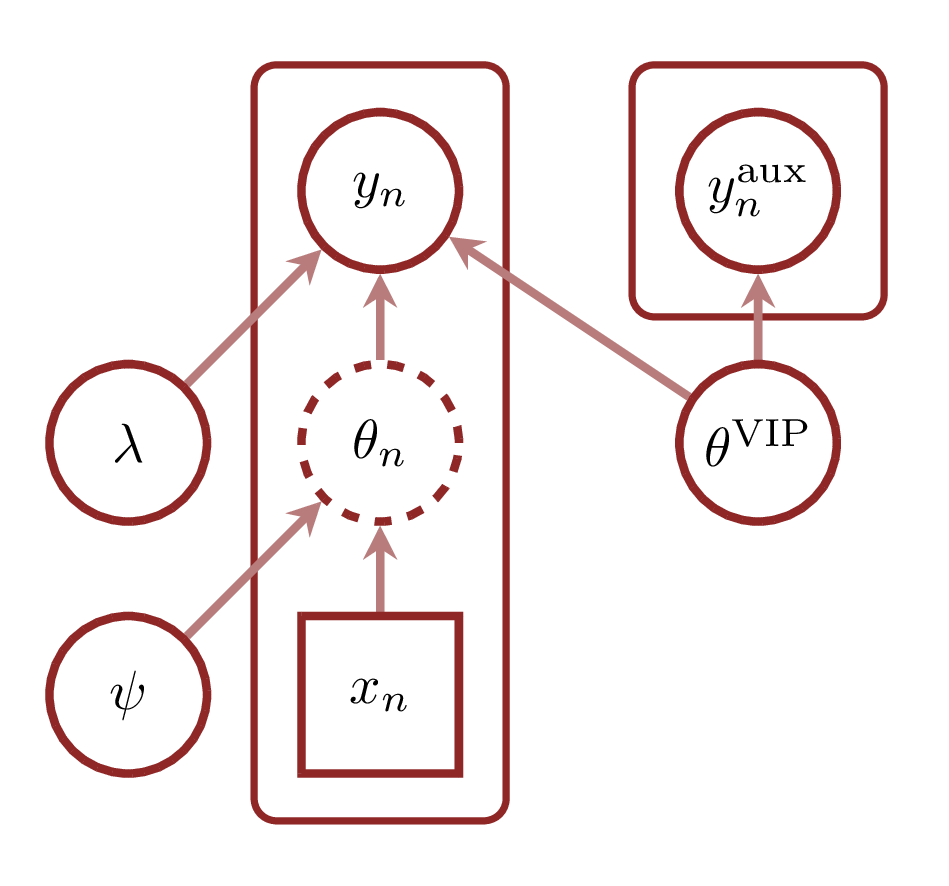
\includegraphics[width=0.5\textwidth,height=\textheight]{figures/4/4.png}

}

\caption{\label{fig-model4}A joint model that incorporates multiple data
generating processes allows us to combine disparate sources of data
together into more precise, but consistent, inferences. Here we combine
our initial observations that could have been generated from one of two
data generating processes with auxiliary observations that are
unambiguously generated from a third data generating process that
depends on only \(\theta^{\text{VIP}}\).}

\end{figure}%

We can now implement this expanded model in the \texttt{Stan} modeling
language, being careful to also include posterior predictions for the
new observations.

\begin{codelisting}

\caption{\texttt{model4.stan}}

\begin{Shaded}
\begin{Highlighting}[]
\KeywordTok{functions}\NormalTok{ \{}
  \CommentTok{// Saturating conversion probability function}
  \DataTypeTok{real}\NormalTok{ theta(}\DataTypeTok{real}\NormalTok{ x, }\DataTypeTok{real}\NormalTok{ psi1, }\DataTypeTok{real}\NormalTok{ psi2) \{}
    \ControlFlowTok{return}\NormalTok{ psi1 * ({-}expm1({-}psi2 * x));}
\NormalTok{  \}}
\NormalTok{\}}

\KeywordTok{data}\NormalTok{ \{}
  \CommentTok{// Observed data}
  \DataTypeTok{int}\NormalTok{\textless{}}\KeywordTok{lower}\NormalTok{=}\DecValTok{1}\NormalTok{\textgreater{} N;                    }\CommentTok{// Number of unique visits}
  \DataTypeTok{array}\NormalTok{[N] }\DataTypeTok{int}\NormalTok{\textless{}}\KeywordTok{lower}\NormalTok{=}\DecValTok{0}\NormalTok{, }\KeywordTok{upper}\NormalTok{=}\DecValTok{1}\NormalTok{\textgreater{} y;  }\CommentTok{// Conversion indicator}
  \DataTypeTok{array}\NormalTok{[N] }\DataTypeTok{real}\NormalTok{ x;                   }\CommentTok{// Previous purchases (USD)}

  \DataTypeTok{int}\NormalTok{\textless{}}\KeywordTok{lower}\NormalTok{=}\DecValTok{1}\NormalTok{\textgreater{} N\_aux;                       }\CommentTok{// Number of VIP{-}only visits}
  \DataTypeTok{array}\NormalTok{[N\_aux] }\DataTypeTok{int}\NormalTok{\textless{}}\KeywordTok{lower}\NormalTok{=}\DecValTok{0}\NormalTok{, }\KeywordTok{upper}\NormalTok{=}\DecValTok{1}\NormalTok{\textgreater{} y\_aux; }\CommentTok{// Conversion indicator}
\NormalTok{\}}

\KeywordTok{parameters}\NormalTok{ \{}
  \DataTypeTok{real}\NormalTok{\textless{}}\KeywordTok{lower}\NormalTok{=}\DecValTok{0}\NormalTok{, }\KeywordTok{upper}\NormalTok{=}\DecValTok{1}\NormalTok{\textgreater{} psi1;      }\CommentTok{// Maximum conversion probability}
  \DataTypeTok{real}\NormalTok{\textless{}}\KeywordTok{lower}\NormalTok{=}\DecValTok{0}\NormalTok{\textgreater{} psi2;               }\CommentTok{// Rate of saturation (1 / kUSD)}
  \DataTypeTok{real}\NormalTok{\textless{}}\KeywordTok{lower}\NormalTok{=}\DecValTok{0}\NormalTok{, }\KeywordTok{upper}\NormalTok{=}\DecValTok{1}\NormalTok{\textgreater{} lambda;    }\CommentTok{// Proportion of VIP visitors}
  \DataTypeTok{real}\NormalTok{\textless{}}\KeywordTok{lower}\NormalTok{=}\DecValTok{0}\NormalTok{, }\KeywordTok{upper}\NormalTok{=}\DecValTok{1}\NormalTok{\textgreater{} theta\_VIP; }\CommentTok{// VIP conversion probability}
\NormalTok{\}}

\KeywordTok{model}\NormalTok{ \{}
  \CommentTok{// Prior model}
\NormalTok{  psi1 \textasciitilde{} beta(}\FloatTok{0.5}\NormalTok{, }\FloatTok{5.0}\NormalTok{);        }\CommentTok{// 0   \textless{}\textasciitilde{}    psi1   \textless{}\textasciitilde{} 0.5}
\NormalTok{  psi2 \textasciitilde{} normal(}\DecValTok{0}\NormalTok{, }\FloatTok{2.0}\NormalTok{ / }\FloatTok{2.57}\NormalTok{); }\CommentTok{// 0   \textless{}\textasciitilde{}    psi2   \textless{}\textasciitilde{} 2}
\NormalTok{  lambda \textasciitilde{} beta(}\DecValTok{1}\NormalTok{, }\DecValTok{1}\NormalTok{);          }\CommentTok{// Uniform probability density function}
\NormalTok{  theta\_VIP \textasciitilde{} beta(}\FloatTok{5.0}\NormalTok{, }\FloatTok{0.5}\NormalTok{);   }\CommentTok{// 0.5 \textless{}\textasciitilde{} theta\_VIP \textless{}\textasciitilde{} 1}

  \CommentTok{// Observational model}
  \ControlFlowTok{for}\NormalTok{ (n }\ControlFlowTok{in} \DecValTok{1}\NormalTok{:N) \{}
    \KeywordTok{target +=}\NormalTok{ log\_mix(lambda,}
\NormalTok{                      bernoulli\_lpmf(y[n] | theta\_VIP),}
\NormalTok{                      bernoulli\_lpmf(y[n] | theta(x[n], psi1, }\FloatTok{1e{-}3}\NormalTok{ * psi2)));}
\NormalTok{  \}}

  \ControlFlowTok{for}\NormalTok{ (n }\ControlFlowTok{in} \DecValTok{1}\NormalTok{:N\_aux) \{}
    \KeywordTok{target +=}\NormalTok{ bernoulli\_lpmf(y\_aux[n] | theta\_VIP);}
\NormalTok{  \}}
\NormalTok{\}}

\KeywordTok{generated quantities}\NormalTok{ \{}
  \CommentTok{// Posterior predictions}
  \DataTypeTok{array}\NormalTok{[N] }\DataTypeTok{real}\NormalTok{ y\_pred;}
  \DataTypeTok{real}\NormalTok{ p\_hat\_pred;}

  \DataTypeTok{array}\NormalTok{[N\_aux] }\DataTypeTok{real}\NormalTok{ y\_aux\_pred;}
  \DataTypeTok{real}\NormalTok{ p\_hat\_aux\_pred;}

  \ControlFlowTok{for}\NormalTok{ (n }\ControlFlowTok{in} \DecValTok{1}\NormalTok{:N) \{}
    \ControlFlowTok{if}\NormalTok{ (bernoulli\_rng(lambda)) \{}
\NormalTok{      y\_pred[n] = bernoulli\_rng(theta\_VIP);}
\NormalTok{    \} }\ControlFlowTok{else}\NormalTok{ \{}
\NormalTok{      y\_pred[n] = bernoulli\_rng(theta(x[n], psi1, }\FloatTok{1e{-}3}\NormalTok{ * psi2));}
\NormalTok{    \}}
\NormalTok{  \}}
\NormalTok{  p\_hat\_pred = mean(y\_pred);}

  \ControlFlowTok{for}\NormalTok{ (n }\ControlFlowTok{in} \DecValTok{1}\NormalTok{:N\_aux) \{}
\NormalTok{    y\_aux\_pred[n] = bernoulli\_rng(theta\_VIP);}
\NormalTok{  \}}
\NormalTok{  p\_hat\_aux\_pred = mean(y\_aux\_pred);}
\NormalTok{\}}
\end{Highlighting}
\end{Shaded}

\end{codelisting}

\begin{Shaded}
\begin{Highlighting}[]
\NormalTok{data }\OtherTok{\textless{}{-}} \FunctionTok{c}\NormalTok{(data, aux\_data)}

\NormalTok{fit }\OtherTok{\textless{}{-}} \FunctionTok{stan}\NormalTok{(}\AttributeTok{file=}\StringTok{"stan\_programs/model4.stan"}\NormalTok{,}
            \AttributeTok{data=}\NormalTok{data, }\AttributeTok{seed=}\DecValTok{8438338}\NormalTok{,}
            \AttributeTok{warmup=}\DecValTok{1000}\NormalTok{, }\AttributeTok{iter=}\DecValTok{2024}\NormalTok{, }\AttributeTok{refresh=}\DecValTok{0}\NormalTok{)}
\end{Highlighting}
\end{Shaded}

Pleasantly we no longer see signs of computational issues when working
with the default adaptation settings. This suggests that the additional
data may indeed have improved the posterior uncertainties.

\begin{Shaded}
\begin{Highlighting}[]
\NormalTok{diagnostics4 }\OtherTok{\textless{}{-}}\NormalTok{ util}\SpecialCharTok{$}\FunctionTok{extract\_hmc\_diagnostics}\NormalTok{(fit)}
\NormalTok{util}\SpecialCharTok{$}\FunctionTok{check\_all\_hmc\_diagnostics}\NormalTok{(diagnostics4)}
\end{Highlighting}
\end{Shaded}

\begin{verbatim}
  All Hamiltonian Monte Carlo diagnostics are consistent with reliable
Markov chain Monte Carlo.
\end{verbatim}

\begin{Shaded}
\begin{Highlighting}[]
\NormalTok{samples4 }\OtherTok{\textless{}{-}}\NormalTok{ util}\SpecialCharTok{$}\FunctionTok{extract\_expectands}\NormalTok{(fit)}
\NormalTok{base\_samples }\OtherTok{\textless{}{-}}\NormalTok{ util}\SpecialCharTok{$}\FunctionTok{filter\_expectands}\NormalTok{(samples4,}
                                       \FunctionTok{c}\NormalTok{(}\StringTok{\textquotesingle{}psi1\textquotesingle{}}\NormalTok{, }\StringTok{\textquotesingle{}psi2\textquotesingle{}}\NormalTok{,}
                                         \StringTok{\textquotesingle{}lambda\textquotesingle{}}\NormalTok{, }\StringTok{\textquotesingle{}theta\_VIP\textquotesingle{}}\NormalTok{))}
\NormalTok{util}\SpecialCharTok{$}\FunctionTok{check\_all\_expectand\_diagnostics}\NormalTok{(base\_samples)}
\end{Highlighting}
\end{Shaded}

\begin{verbatim}
All expectands checked appear to be behaving well enough for reliable
Markov chain Monte Carlo estimation.
\end{verbatim}

None of our visual retrodictive checks indicate any model inadequacies,
including the aggregate conversion frequency of the newly incorporated
data.

\begin{Shaded}
\begin{Highlighting}[]
\FunctionTok{par}\NormalTok{(}\AttributeTok{mfrow=}\FunctionTok{c}\NormalTok{(}\DecValTok{1}\NormalTok{, }\DecValTok{2}\NormalTok{), }\AttributeTok{mar=}\FunctionTok{c}\NormalTok{(}\DecValTok{5}\NormalTok{, }\DecValTok{5}\NormalTok{, }\DecValTok{3}\NormalTok{, }\DecValTok{1}\NormalTok{))}

\NormalTok{util}\SpecialCharTok{$}\FunctionTok{plot\_expectand\_pushforward}\NormalTok{(samples4[[}\StringTok{\textquotesingle{}p\_hat\_pred\textquotesingle{}}\NormalTok{]], }\DecValTok{20}\NormalTok{,}
                                \AttributeTok{display\_name=}\StringTok{"Aggregate Conversion Frequency"}\NormalTok{,}
                                \AttributeTok{baseline=}\FunctionTok{mean}\NormalTok{(data}\SpecialCharTok{$}\NormalTok{y),}
                                \AttributeTok{main=}\StringTok{"Main Observations"}\NormalTok{)}

\NormalTok{util}\SpecialCharTok{$}\FunctionTok{plot\_expectand\_pushforward}\NormalTok{(samples4[[}\StringTok{\textquotesingle{}p\_hat\_aux\_pred\textquotesingle{}}\NormalTok{]], }\DecValTok{10}\NormalTok{,}
                                \AttributeTok{display\_name=}\StringTok{"Aggregate Conversion Frequency"}\NormalTok{,}
                                \AttributeTok{baseline=}\FunctionTok{mean}\NormalTok{(data}\SpecialCharTok{$}\NormalTok{y\_aux),}
                                \AttributeTok{main=}\StringTok{"Auxililary Observations"}\NormalTok{)}
\end{Highlighting}
\end{Shaded}

\includegraphics{customer_conversion_files/figure-pdf/unnamed-chunk-39-1.pdf}

\begin{Shaded}
\begin{Highlighting}[]
\FunctionTok{par}\NormalTok{(}\AttributeTok{mfrow=}\FunctionTok{c}\NormalTok{(}\DecValTok{1}\NormalTok{, }\DecValTok{1}\NormalTok{), }\AttributeTok{mar=}\FunctionTok{c}\NormalTok{(}\DecValTok{5}\NormalTok{, }\DecValTok{5}\NormalTok{, }\DecValTok{3}\NormalTok{, }\DecValTok{1}\NormalTok{))}

\NormalTok{pred\_names }\OtherTok{\textless{}{-}} \FunctionTok{sapply}\NormalTok{(}\DecValTok{1}\SpecialCharTok{:}\NormalTok{data}\SpecialCharTok{$}\NormalTok{N, }\ControlFlowTok{function}\NormalTok{(n) }\FunctionTok{paste0}\NormalTok{(}\StringTok{\textquotesingle{}y\_pred[\textquotesingle{}}\NormalTok{, n, }\StringTok{\textquotesingle{}]\textquotesingle{}}\NormalTok{))}
\NormalTok{util}\SpecialCharTok{$}\FunctionTok{plot\_conditional\_mean\_quantiles}\NormalTok{(samples4, pred\_names, data}\SpecialCharTok{$}\NormalTok{x,}
                                     \DecValTok{0}\NormalTok{, }\DecValTok{6120}\NormalTok{, }\DecValTok{153}\NormalTok{,}
                                     \AttributeTok{baseline\_values=}\NormalTok{data}\SpecialCharTok{$}\NormalTok{y,}
                                     \AttributeTok{xlab=}\StringTok{"Previous Purchases (USD)"}\NormalTok{,}
                                     \AttributeTok{ylab=}\StringTok{"Binned Conversion Frequency"}\NormalTok{)}
\end{Highlighting}
\end{Shaded}

\includegraphics{customer_conversion_files/figure-pdf/unnamed-chunk-40-1.pdf}

Have our posterior uncertainties actually been reduced by the addition
of these auxiliary observations? The marginal posterior inferences for
\(\psi_{1}\) and \(\psi_{2}\) are similar to what we encountered
previously.

\begin{Shaded}
\begin{Highlighting}[]
\FunctionTok{par}\NormalTok{(}\AttributeTok{mfrow=}\FunctionTok{c}\NormalTok{(}\DecValTok{2}\NormalTok{, }\DecValTok{2}\NormalTok{), }\AttributeTok{mar=}\FunctionTok{c}\NormalTok{(}\DecValTok{5}\NormalTok{, }\DecValTok{5}\NormalTok{, }\DecValTok{2}\NormalTok{, }\DecValTok{1}\NormalTok{))}

\NormalTok{util}\SpecialCharTok{$}\FunctionTok{plot\_expectand\_pushforward}\NormalTok{(samples3\_99[[}\StringTok{\textquotesingle{}psi1\textquotesingle{}}\NormalTok{]], }\DecValTok{50}\NormalTok{,}
                                \AttributeTok{display\_name=}\StringTok{"psi1"}\NormalTok{,}
                                \AttributeTok{flim=}\FunctionTok{c}\NormalTok{(}\DecValTok{0}\NormalTok{, }\DecValTok{1}\NormalTok{),}
                                \AttributeTok{main=}\StringTok{"Model 3"}\NormalTok{)}
\NormalTok{xs }\OtherTok{\textless{}{-}} \FunctionTok{seq}\NormalTok{(}\DecValTok{0}\NormalTok{, }\DecValTok{1}\NormalTok{, }\FloatTok{0.01}\NormalTok{)}
\FunctionTok{lines}\NormalTok{(xs, }\FunctionTok{dbeta}\NormalTok{(xs, }\FloatTok{0.5}\NormalTok{, }\FloatTok{5.0}\NormalTok{), }\AttributeTok{lwd=}\DecValTok{2}\NormalTok{, }\AttributeTok{col=}\NormalTok{util}\SpecialCharTok{$}\NormalTok{c\_mid\_teal)}

\NormalTok{util}\SpecialCharTok{$}\FunctionTok{plot\_expectand\_pushforward}\NormalTok{(samples4[[}\StringTok{\textquotesingle{}psi1\textquotesingle{}}\NormalTok{]], }\DecValTok{50}\NormalTok{,}
                                \AttributeTok{display\_name=}\StringTok{"psi1"}\NormalTok{,}
                                \AttributeTok{flim=}\FunctionTok{c}\NormalTok{(}\DecValTok{0}\NormalTok{, }\DecValTok{1}\NormalTok{),}
                                \AttributeTok{main=}\StringTok{"Model 4"}\NormalTok{)}
\NormalTok{xs }\OtherTok{\textless{}{-}} \FunctionTok{seq}\NormalTok{(}\DecValTok{0}\NormalTok{, }\DecValTok{1}\NormalTok{, }\FloatTok{0.01}\NormalTok{)}
\FunctionTok{lines}\NormalTok{(xs, }\FunctionTok{dbeta}\NormalTok{(xs, }\FloatTok{0.5}\NormalTok{, }\FloatTok{5.0}\NormalTok{), }\AttributeTok{lwd=}\DecValTok{2}\NormalTok{, }\AttributeTok{col=}\NormalTok{util}\SpecialCharTok{$}\NormalTok{c\_mid\_teal)}

\NormalTok{util}\SpecialCharTok{$}\FunctionTok{plot\_expectand\_pushforward}\NormalTok{(samples3\_99[[}\StringTok{\textquotesingle{}psi2\textquotesingle{}}\NormalTok{]], }\DecValTok{30}\NormalTok{,}
                                \AttributeTok{display\_name=}\StringTok{"psi2"}\NormalTok{,}
                                \AttributeTok{flim=}\FunctionTok{c}\NormalTok{(}\DecValTok{0}\NormalTok{, }\DecValTok{4}\NormalTok{),}
                                \AttributeTok{main=}\StringTok{"Model 3"}\NormalTok{)}
\NormalTok{xs }\OtherTok{\textless{}{-}} \FunctionTok{seq}\NormalTok{(}\DecValTok{0}\NormalTok{, }\DecValTok{4}\NormalTok{, }\FloatTok{0.05}\NormalTok{)}
\FunctionTok{lines}\NormalTok{(xs, }\DecValTok{2} \SpecialCharTok{*} \FunctionTok{dnorm}\NormalTok{(xs, }\DecValTok{0}\NormalTok{, }\FloatTok{2.0} \SpecialCharTok{/} \FloatTok{2.57}\NormalTok{), }\AttributeTok{lwd=}\DecValTok{2}\NormalTok{, }\AttributeTok{col=}\NormalTok{util}\SpecialCharTok{$}\NormalTok{c\_mid\_teal)}

\NormalTok{util}\SpecialCharTok{$}\FunctionTok{plot\_expectand\_pushforward}\NormalTok{(samples4[[}\StringTok{\textquotesingle{}psi2\textquotesingle{}}\NormalTok{]], }\DecValTok{30}\NormalTok{,}
                                \AttributeTok{display\_name=}\StringTok{"psi2"}\NormalTok{,}
                                \AttributeTok{flim=}\FunctionTok{c}\NormalTok{(}\DecValTok{0}\NormalTok{, }\DecValTok{4}\NormalTok{),}
                                \AttributeTok{main=}\StringTok{"Model 4"}\NormalTok{)}
\NormalTok{xs }\OtherTok{\textless{}{-}} \FunctionTok{seq}\NormalTok{(}\DecValTok{0}\NormalTok{, }\DecValTok{4}\NormalTok{, }\FloatTok{0.05}\NormalTok{)}
\FunctionTok{lines}\NormalTok{(xs, }\DecValTok{2} \SpecialCharTok{*} \FunctionTok{dnorm}\NormalTok{(xs, }\DecValTok{0}\NormalTok{, }\FloatTok{2.0} \SpecialCharTok{/} \FloatTok{2.57}\NormalTok{), }\AttributeTok{lwd=}\DecValTok{2}\NormalTok{, }\AttributeTok{col=}\NormalTok{util}\SpecialCharTok{$}\NormalTok{c\_mid\_teal)}
\end{Highlighting}
\end{Shaded}

\includegraphics{customer_conversion_files/figure-pdf/unnamed-chunk-41-1.pdf}

Looking at the corresponding pairs plot we can see that there are many
different configurations of the conversion probability function
consistent with the observed data and our domain expertise: larger
maximum conversion probabilities can be accommodated by reducing the
speed of saturation and vice versa. In order to better inform these two
parameters we would probably need to collect more conversion data at
larger previous purchases.

\begin{Shaded}
\begin{Highlighting}[]
\FunctionTok{par}\NormalTok{(}\AttributeTok{mfrow=}\FunctionTok{c}\NormalTok{(}\DecValTok{1}\NormalTok{, }\DecValTok{1}\NormalTok{))}

\FunctionTok{plot}\NormalTok{(}\FunctionTok{c}\NormalTok{(samples4[}\StringTok{\textquotesingle{}psi1\textquotesingle{}}\NormalTok{], }\AttributeTok{recursive=}\ConstantTok{TRUE}\NormalTok{),}
     \FunctionTok{c}\NormalTok{(samples4[}\StringTok{\textquotesingle{}psi2\textquotesingle{}}\NormalTok{], }\AttributeTok{recursive=}\ConstantTok{TRUE}\NormalTok{),}
     \AttributeTok{col=}\NormalTok{util}\SpecialCharTok{$}\NormalTok{c\_dark, }\AttributeTok{pch=}\DecValTok{16}\NormalTok{, }\AttributeTok{cex=}\FloatTok{0.8}\NormalTok{,}
     \AttributeTok{xlab=}\StringTok{"psi1"}\NormalTok{, }\AttributeTok{ylab=}\StringTok{"psi2"}\NormalTok{)}
\end{Highlighting}
\end{Shaded}

\includegraphics{customer_conversion_files/figure-pdf/unnamed-chunk-42-1.pdf}

On the other hand the marginal posterior distribution for \(\lambda\)
suppresses large values than before.

\begin{Shaded}
\begin{Highlighting}[]
\FunctionTok{par}\NormalTok{(}\AttributeTok{mfrow=}\FunctionTok{c}\NormalTok{(}\DecValTok{1}\NormalTok{, }\DecValTok{2}\NormalTok{), }\AttributeTok{mar=}\FunctionTok{c}\NormalTok{(}\DecValTok{5}\NormalTok{, }\DecValTok{5}\NormalTok{, }\DecValTok{2}\NormalTok{, }\DecValTok{1}\NormalTok{))}

\NormalTok{util}\SpecialCharTok{$}\FunctionTok{plot\_expectand\_pushforward}\NormalTok{(samples3\_99[[}\StringTok{\textquotesingle{}lambda\textquotesingle{}}\NormalTok{]], }\DecValTok{50}\NormalTok{,}
                                \AttributeTok{display\_name=}\StringTok{"lambda"}\NormalTok{,}
                                \AttributeTok{flim=}\FunctionTok{c}\NormalTok{(}\DecValTok{0}\NormalTok{, }\DecValTok{1}\NormalTok{),}
                                \AttributeTok{main=}\StringTok{"Model 3"}\NormalTok{)}
\NormalTok{xs }\OtherTok{\textless{}{-}} \FunctionTok{seq}\NormalTok{(}\DecValTok{0}\NormalTok{, }\DecValTok{1}\NormalTok{, }\FloatTok{0.01}\NormalTok{)}
\FunctionTok{lines}\NormalTok{(xs, }\FunctionTok{dbeta}\NormalTok{(xs, }\DecValTok{1}\NormalTok{, }\DecValTok{1}\NormalTok{), }\AttributeTok{lwd=}\DecValTok{2}\NormalTok{, }\AttributeTok{col=}\NormalTok{util}\SpecialCharTok{$}\NormalTok{c\_mid\_teal)}

\NormalTok{util}\SpecialCharTok{$}\FunctionTok{plot\_expectand\_pushforward}\NormalTok{(samples4[[}\StringTok{\textquotesingle{}lambda\textquotesingle{}}\NormalTok{]], }\DecValTok{50}\NormalTok{,}
                                \AttributeTok{display\_name=}\StringTok{"lambda"}\NormalTok{,}
                                \AttributeTok{flim=}\FunctionTok{c}\NormalTok{(}\DecValTok{0}\NormalTok{, }\DecValTok{1}\NormalTok{),}
                                \AttributeTok{main=}\StringTok{"Model 4"}\NormalTok{)}
\NormalTok{xs }\OtherTok{\textless{}{-}} \FunctionTok{seq}\NormalTok{(}\DecValTok{0}\NormalTok{, }\DecValTok{1}\NormalTok{, }\FloatTok{0.01}\NormalTok{)}
\FunctionTok{lines}\NormalTok{(xs, }\FunctionTok{dbeta}\NormalTok{(xs, }\DecValTok{1}\NormalTok{, }\DecValTok{1}\NormalTok{), }\AttributeTok{lwd=}\DecValTok{2}\NormalTok{, }\AttributeTok{col=}\NormalTok{util}\SpecialCharTok{$}\NormalTok{c\_mid\_teal)}
\end{Highlighting}
\end{Shaded}

\includegraphics{customer_conversion_files/figure-pdf/unnamed-chunk-43-1.pdf}

More importantly the marginal posterior distribution for
\(\theta^{\text{VIP}}\) now strongly contracts away from the prior
model.

\begin{Shaded}
\begin{Highlighting}[]
\FunctionTok{par}\NormalTok{(}\AttributeTok{mfrow=}\FunctionTok{c}\NormalTok{(}\DecValTok{1}\NormalTok{, }\DecValTok{2}\NormalTok{), }\AttributeTok{mar=}\FunctionTok{c}\NormalTok{(}\DecValTok{5}\NormalTok{, }\DecValTok{5}\NormalTok{, }\DecValTok{2}\NormalTok{, }\DecValTok{1}\NormalTok{))}
\NormalTok{util}\SpecialCharTok{$}\FunctionTok{plot\_expectand\_pushforward}\NormalTok{(samples3\_99[[}\StringTok{\textquotesingle{}theta\_VIP\textquotesingle{}}\NormalTok{]], }\DecValTok{50}\NormalTok{,}
                                \AttributeTok{display\_name=}\StringTok{"theta\_VIP"}\NormalTok{,}
                                \AttributeTok{flim=}\FunctionTok{c}\NormalTok{(}\DecValTok{0}\NormalTok{, }\DecValTok{1}\NormalTok{),}
                                \AttributeTok{main=}\StringTok{"Model 3"}\NormalTok{)}
\NormalTok{xs }\OtherTok{\textless{}{-}} \FunctionTok{seq}\NormalTok{(}\DecValTok{0}\NormalTok{, }\DecValTok{1}\NormalTok{, }\FloatTok{0.01}\NormalTok{)}
\FunctionTok{lines}\NormalTok{(xs, }\FunctionTok{dbeta}\NormalTok{(xs, }\FloatTok{5.0}\NormalTok{, }\FloatTok{0.5}\NormalTok{), }\AttributeTok{lwd=}\DecValTok{2}\NormalTok{, }\AttributeTok{col=}\NormalTok{util}\SpecialCharTok{$}\NormalTok{c\_mid\_teal)}

\NormalTok{util}\SpecialCharTok{$}\FunctionTok{plot\_expectand\_pushforward}\NormalTok{(samples4[[}\StringTok{\textquotesingle{}theta\_VIP\textquotesingle{}}\NormalTok{]], }\DecValTok{50}\NormalTok{,}
                                \AttributeTok{display\_name=}\StringTok{"theta\_VIP"}\NormalTok{,}
                                \AttributeTok{flim=}\FunctionTok{c}\NormalTok{(}\DecValTok{0}\NormalTok{, }\DecValTok{1}\NormalTok{),}
                                \AttributeTok{main=}\StringTok{"Model 4"}\NormalTok{)}
\NormalTok{xs }\OtherTok{\textless{}{-}} \FunctionTok{seq}\NormalTok{(}\DecValTok{0}\NormalTok{, }\DecValTok{1}\NormalTok{, }\FloatTok{0.01}\NormalTok{)}
\FunctionTok{lines}\NormalTok{(xs, }\FunctionTok{dbeta}\NormalTok{(xs, }\FloatTok{5.0}\NormalTok{, }\FloatTok{0.5}\NormalTok{), }\AttributeTok{lwd=}\DecValTok{2}\NormalTok{, }\AttributeTok{col=}\NormalTok{util}\SpecialCharTok{$}\NormalTok{c\_mid\_teal)}
\end{Highlighting}
\end{Shaded}

\includegraphics{customer_conversion_files/figure-pdf/unnamed-chunk-44-1.pdf}

\subsection{Hypothetical Predictions}\label{hypothetical-predictions}

Now that we can reasonably disentangle all of the data generating
behaviors we can use them to inform inferences, decisions, and
predictions about new circumstances. These tasks are ubiquitous in both
science and industry but they are denoted by a wildly confusing array of
adjectives, such as hypothetical, counterfactual, out-of-sample,
generalized, and the like.

For example let's say that we want to understand what would happen if we
could redesign the customer experience to exclude VIP customers
entirely. In this case the behavior of the regular customers would not
be properly modeled by \[
\text{Bernoulli} \, (y_{n} \mid \theta \, (x_{n}, \psi))
+ (1 - \lambda) \cdot
\text{Bernoulli} \, (y_{n} \mid \theta^{\text{VIP}})
\] nor \[
\text{Bernoulli} \, (y^{\text{aux}}_{n} \mid \theta^{\text{VIP}})
\] but rather \[
\text{Bernoulli} \, (y_{n} \mid \theta \, (x_{n}, \psi)).
\] Fortunately we can readily expand our model to accommodate this new
behavior (Figure~\ref{fig-model5}).

\begin{figure}

\centering{

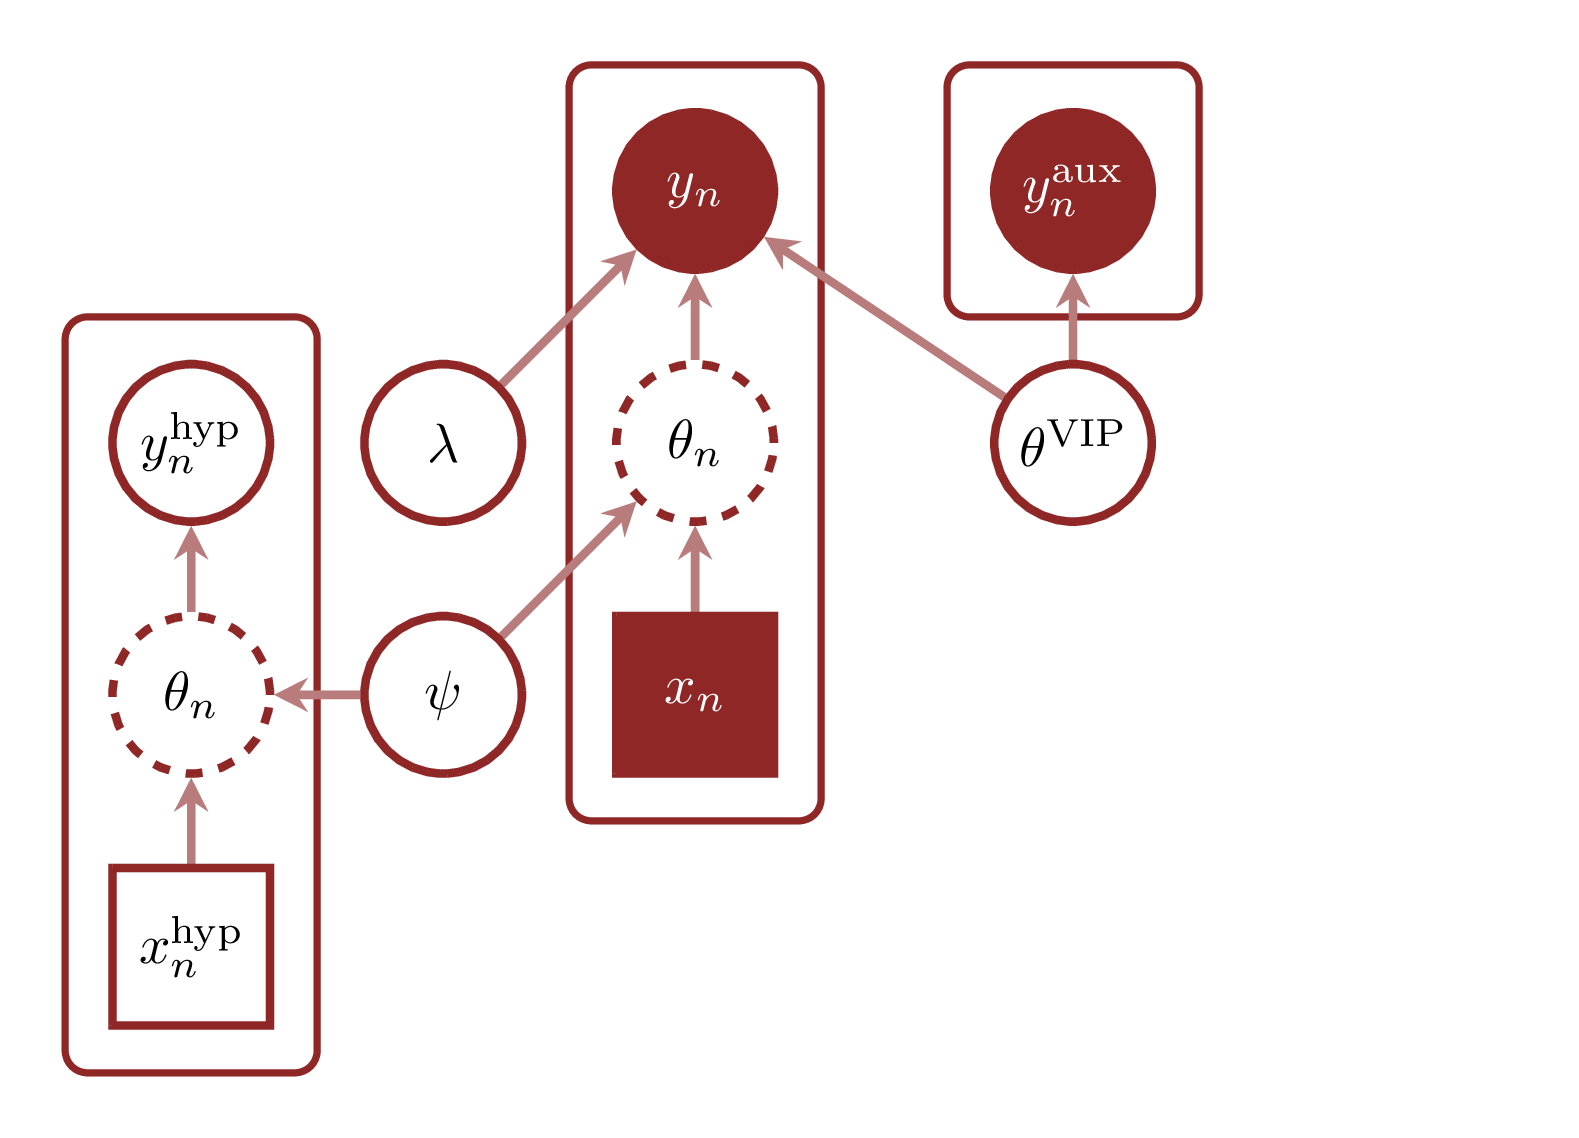
\includegraphics[width=0.83\textwidth,height=\textheight]{figures/6/6.png}

}

\caption{\label{fig-model5}Narratively generative modeling allows us to
consider not just the data generating processes responsible for observed
data but also those that might be responsible for data to which we do
not yet have access, such as the observations that would be generated by
hypothetical or future measurements.}

\end{figure}%

In order to actually implement these new, hypothetical predictions we
need to determine appropriate values for the previous purchases. This is
complicated by the fact that we have been explicitly modeling these
values! Although this might initially come across as a burden it can
actually be a really useful opportunity. For example if we want to
analyze the behavior across all possible previous purchases we can
select previous purchases from a uniform grid of values.

\begin{Shaded}
\begin{Highlighting}[]
\NormalTok{x\_grid }\OtherTok{\textless{}{-}} \FunctionTok{seq}\NormalTok{(}\DecValTok{0}\NormalTok{, }\DecValTok{5000}\NormalTok{, }\DecValTok{125}\NormalTok{)}
\NormalTok{data}\SpecialCharTok{$}\NormalTok{N\_hyp }\OtherTok{\textless{}{-}} \DecValTok{2050}
\NormalTok{data}\SpecialCharTok{$}\NormalTok{x\_hyp }\OtherTok{\textless{}{-}} \FunctionTok{rep}\NormalTok{(x\_grid, }\AttributeTok{each=}\DecValTok{50}\NormalTok{)}
\end{Highlighting}
\end{Shaded}

Incorporating these new predictions into a \texttt{Stan} program just
requires expanding the \texttt{data} and \texttt{generated\ quantities}
blocks. The \texttt{parameters} and \texttt{model} blocks remain exactly
the same. We are not changing our inferences, just what we do with that
information.

\begin{codelisting}

\caption{\texttt{model5.stan}}

\begin{Shaded}
\begin{Highlighting}[]
\KeywordTok{functions}\NormalTok{ \{}
  \CommentTok{// Saturating conversion probability function}
  \DataTypeTok{real}\NormalTok{ theta(}\DataTypeTok{real}\NormalTok{ x, }\DataTypeTok{real}\NormalTok{ psi1, }\DataTypeTok{real}\NormalTok{ psi2) \{}
    \ControlFlowTok{return}\NormalTok{ psi1 * ({-}expm1({-}psi2 * x));}
\NormalTok{  \}}
\NormalTok{\}}

\KeywordTok{data}\NormalTok{ \{}
  \CommentTok{// Observed data}
  \DataTypeTok{int}\NormalTok{\textless{}}\KeywordTok{lower}\NormalTok{=}\DecValTok{1}\NormalTok{\textgreater{} N;                    }\CommentTok{// Number of unique visits}
  \DataTypeTok{array}\NormalTok{[N] }\DataTypeTok{int}\NormalTok{\textless{}}\KeywordTok{lower}\NormalTok{=}\DecValTok{0}\NormalTok{, }\KeywordTok{upper}\NormalTok{=}\DecValTok{1}\NormalTok{\textgreater{} y;  }\CommentTok{// Conversion indicator}
  \DataTypeTok{array}\NormalTok{[N] }\DataTypeTok{real}\NormalTok{ x;                   }\CommentTok{// Previous purchases (USD)}

  \DataTypeTok{int}\NormalTok{\textless{}}\KeywordTok{lower}\NormalTok{=}\DecValTok{1}\NormalTok{\textgreater{} N\_aux;                       }\CommentTok{// Number of VIP{-}only visits}
  \DataTypeTok{array}\NormalTok{[N\_aux] }\DataTypeTok{int}\NormalTok{\textless{}}\KeywordTok{lower}\NormalTok{=}\DecValTok{0}\NormalTok{, }\KeywordTok{upper}\NormalTok{=}\DecValTok{1}\NormalTok{\textgreater{} y\_aux; }\CommentTok{// Conversion indicator}

  \CommentTok{// Hypothetical data}
  \DataTypeTok{int}\NormalTok{\textless{}}\KeywordTok{lower}\NormalTok{=}\DecValTok{1}\NormalTok{\textgreater{} N\_hyp;}
  \DataTypeTok{array}\NormalTok{[N\_hyp] }\DataTypeTok{real}\NormalTok{ x\_hyp;}
\NormalTok{\}}

\KeywordTok{parameters}\NormalTok{ \{}
  \DataTypeTok{real}\NormalTok{\textless{}}\KeywordTok{lower}\NormalTok{=}\DecValTok{0}\NormalTok{, }\KeywordTok{upper}\NormalTok{=}\DecValTok{1}\NormalTok{\textgreater{} psi1;      }\CommentTok{// Maximum conversion probability}
  \DataTypeTok{real}\NormalTok{\textless{}}\KeywordTok{lower}\NormalTok{=}\DecValTok{0}\NormalTok{\textgreater{} psi2;               }\CommentTok{// Rate of saturation (1 / kUSD)}
  \DataTypeTok{real}\NormalTok{\textless{}}\KeywordTok{lower}\NormalTok{=}\DecValTok{0}\NormalTok{, }\KeywordTok{upper}\NormalTok{=}\DecValTok{1}\NormalTok{\textgreater{} lambda;    }\CommentTok{// Proportion of VIP visitors}
  \DataTypeTok{real}\NormalTok{\textless{}}\KeywordTok{lower}\NormalTok{=}\DecValTok{0}\NormalTok{, }\KeywordTok{upper}\NormalTok{=}\DecValTok{1}\NormalTok{\textgreater{} theta\_VIP; }\CommentTok{// VIP conversion probability}
\NormalTok{\}}

\KeywordTok{model}\NormalTok{ \{}
  \CommentTok{// Prior model}
\NormalTok{  psi1 \textasciitilde{} beta(}\FloatTok{0.5}\NormalTok{, }\FloatTok{5.0}\NormalTok{);        }\CommentTok{// 0   \textless{}\textasciitilde{}    psi1   \textless{}\textasciitilde{} 0.5}
\NormalTok{  psi2 \textasciitilde{} normal(}\DecValTok{0}\NormalTok{, }\FloatTok{2.0}\NormalTok{ / }\FloatTok{2.57}\NormalTok{); }\CommentTok{// 0   \textless{}\textasciitilde{}    psi2   \textless{}\textasciitilde{} 2}
\NormalTok{  lambda \textasciitilde{} beta(}\DecValTok{1}\NormalTok{, }\DecValTok{1}\NormalTok{);          }\CommentTok{// Uniform probability density function}
\NormalTok{  theta\_VIP \textasciitilde{} beta(}\FloatTok{5.0}\NormalTok{, }\FloatTok{0.5}\NormalTok{);   }\CommentTok{// 0.5 \textless{}\textasciitilde{} theta\_VIP \textless{}\textasciitilde{} 1}

  \CommentTok{// Observational model}
  \ControlFlowTok{for}\NormalTok{ (n }\ControlFlowTok{in} \DecValTok{1}\NormalTok{:N) \{}
    \KeywordTok{target +=}\NormalTok{ log\_mix(lambda,}
\NormalTok{                      bernoulli\_lpmf(y[n] | theta\_VIP),}
\NormalTok{                      bernoulli\_lpmf(y[n] | theta(x[n], psi1, }\FloatTok{1e{-}3}\NormalTok{ * psi2)));}
\NormalTok{  \}}

  \ControlFlowTok{for}\NormalTok{ (n }\ControlFlowTok{in} \DecValTok{1}\NormalTok{:N\_aux) \{}
    \KeywordTok{target +=}\NormalTok{ bernoulli\_lpmf(y\_aux[n] | theta\_VIP);}
\NormalTok{  \}}
\NormalTok{\}}

\KeywordTok{generated quantities}\NormalTok{ \{}
  \CommentTok{// Posterior predictions}
  \DataTypeTok{array}\NormalTok{[N] }\DataTypeTok{real}\NormalTok{ y\_pred;}
  \DataTypeTok{array}\NormalTok{[N\_aux] }\DataTypeTok{real}\NormalTok{ y\_aux\_pred;}
  \DataTypeTok{array}\NormalTok{[N\_hyp] }\DataTypeTok{real}\NormalTok{ y\_hyp\_pred;}

  \ControlFlowTok{for}\NormalTok{ (n }\ControlFlowTok{in} \DecValTok{1}\NormalTok{:N) \{}
    \ControlFlowTok{if}\NormalTok{ (bernoulli\_rng(lambda)) \{}
\NormalTok{      y\_pred[n] = bernoulli\_rng(theta\_VIP);}
\NormalTok{    \} }\ControlFlowTok{else}\NormalTok{ \{}
\NormalTok{      y\_pred[n] = bernoulli\_rng(theta(x[n], psi1, }\FloatTok{1e{-}3}\NormalTok{ * psi2));}
\NormalTok{    \}}
\NormalTok{  \}}

  \ControlFlowTok{for}\NormalTok{ (n }\ControlFlowTok{in} \DecValTok{1}\NormalTok{:N\_aux) \{}
\NormalTok{    y\_aux\_pred[n] = bernoulli\_rng(theta\_VIP);}
\NormalTok{  \}}

  \ControlFlowTok{for}\NormalTok{ (n }\ControlFlowTok{in} \DecValTok{1}\NormalTok{:N\_hyp) \{}
\NormalTok{    y\_hyp\_pred[n] = bernoulli\_rng(theta(x\_hyp[n], psi1, }\FloatTok{1e{-}3}\NormalTok{ * psi2));}
\NormalTok{  \}}
\NormalTok{\}}
\end{Highlighting}
\end{Shaded}

\end{codelisting}

\begin{Shaded}
\begin{Highlighting}[]
\NormalTok{fit }\OtherTok{\textless{}{-}} \FunctionTok{stan}\NormalTok{(}\AttributeTok{file=}\StringTok{"stan\_programs/model5.stan"}\NormalTok{,}
            \AttributeTok{data=}\NormalTok{data, }\AttributeTok{seed=}\DecValTok{8438338}\NormalTok{,}
            \AttributeTok{warmup=}\DecValTok{1000}\NormalTok{, }\AttributeTok{iter=}\DecValTok{2024}\NormalTok{, }\AttributeTok{refresh=}\DecValTok{0}\NormalTok{)}

\NormalTok{samples5 }\OtherTok{\textless{}{-}}\NormalTok{ util}\SpecialCharTok{$}\FunctionTok{extract\_expectands}\NormalTok{(fit)}
\end{Highlighting}
\end{Shaded}

Because we are effectively rerunning the same computation we don't need
to check the computational diagnostics nor the posterior retrodictive
checks.

As expected our predictions for the new circumstances don't look like
any of our retrodictions. The hypothetical data generating process
yields conversion frequencies that increase but quickly saturate with
increasing previous purchases but are not contaminated by VIP customers.
This results in conversion frequencies that vary with previous purchases
but are uniformly smaller than what we see in the observed data.

\begin{Shaded}
\begin{Highlighting}[]
\FunctionTok{par}\NormalTok{(}\AttributeTok{mfrow=}\FunctionTok{c}\NormalTok{(}\DecValTok{1}\NormalTok{, }\DecValTok{3}\NormalTok{), }\AttributeTok{mar=}\FunctionTok{c}\NormalTok{(}\DecValTok{5}\NormalTok{, }\DecValTok{5}\NormalTok{, }\DecValTok{3}\NormalTok{, }\DecValTok{1}\NormalTok{))}

\NormalTok{pred\_names }\OtherTok{\textless{}{-}} \FunctionTok{sapply}\NormalTok{(}\DecValTok{1}\SpecialCharTok{:}\NormalTok{data}\SpecialCharTok{$}\NormalTok{N, }\ControlFlowTok{function}\NormalTok{(n) }\FunctionTok{paste0}\NormalTok{(}\StringTok{\textquotesingle{}y\_pred[\textquotesingle{}}\NormalTok{, n, }\StringTok{\textquotesingle{}]\textquotesingle{}}\NormalTok{))}
\NormalTok{util}\SpecialCharTok{$}\FunctionTok{plot\_conditional\_mean\_quantiles}\NormalTok{(samples5, pred\_names, data}\SpecialCharTok{$}\NormalTok{x,}
                                     \DecValTok{0}\NormalTok{, }\DecValTok{5000}\NormalTok{, }\DecValTok{150}\NormalTok{,}
                                     \AttributeTok{xlab=}\StringTok{"Previous Purchases (USD)"}\NormalTok{,}
                                     \AttributeTok{ylab=}\StringTok{"Binned Conversion Frequency"}\NormalTok{,}
                                     \AttributeTok{display\_ylim=}\FunctionTok{c}\NormalTok{(}\DecValTok{0}\NormalTok{, }\DecValTok{1}\NormalTok{),}
                                     \AttributeTok{main=}\StringTok{"Main Retrodictions"}\NormalTok{)}
\end{Highlighting}
\end{Shaded}

\begin{verbatim}
Warning in check_bin_containment(bin_min, bin_max, obs_xs, "conditioning
value"): 6 conditioning values (0.4%) fell above the binning.
\end{verbatim}

\begin{Shaded}
\begin{Highlighting}[]
\NormalTok{pred\_names }\OtherTok{\textless{}{-}} \FunctionTok{sapply}\NormalTok{(}\DecValTok{1}\SpecialCharTok{:}\NormalTok{data}\SpecialCharTok{$}\NormalTok{N\_aux, }\ControlFlowTok{function}\NormalTok{(n) }\FunctionTok{paste0}\NormalTok{(}\StringTok{\textquotesingle{}y\_aux\_pred[\textquotesingle{}}\NormalTok{, n, }\StringTok{\textquotesingle{}]\textquotesingle{}}\NormalTok{))}
\NormalTok{probs }\OtherTok{\textless{}{-}} \FunctionTok{c}\NormalTok{(}\FloatTok{0.1}\NormalTok{, }\FloatTok{0.2}\NormalTok{, }\FloatTok{0.3}\NormalTok{, }\FloatTok{0.4}\NormalTok{, }\FloatTok{0.5}\NormalTok{, }\FloatTok{0.6}\NormalTok{, }\FloatTok{0.7}\NormalTok{, }\FloatTok{0.8}\NormalTok{, }\FloatTok{0.9}\NormalTok{)}

\NormalTok{mean\_quantiles }\OtherTok{\textless{}{-}} \FunctionTok{rep}\NormalTok{(}\DecValTok{0}\NormalTok{, }\DecValTok{9}\NormalTok{)}
\ControlFlowTok{for}\NormalTok{ (c }\ControlFlowTok{in} \DecValTok{1}\SpecialCharTok{:}\DecValTok{4}\NormalTok{) \{}
\NormalTok{  values }\OtherTok{\textless{}{-}} \FunctionTok{t}\NormalTok{(}\FunctionTok{sapply}\NormalTok{(pred\_names, }\ControlFlowTok{function}\NormalTok{(name) samples5[[name]][c,]))}
\NormalTok{  means }\OtherTok{\textless{}{-}} \FunctionTok{sapply}\NormalTok{(}\DecValTok{1}\SpecialCharTok{:}\DecValTok{1024}\NormalTok{, }\ControlFlowTok{function}\NormalTok{(s) }\FunctionTok{mean}\NormalTok{(values[,s]))}
\NormalTok{  mean\_quantiles }\OtherTok{\textless{}{-}}\NormalTok{ mean\_quantiles }\SpecialCharTok{+} \FunctionTok{quantile}\NormalTok{(means, }\AttributeTok{probs=}\NormalTok{probs) }\SpecialCharTok{/} \DecValTok{4}
\NormalTok{\}}

\FunctionTok{plot}\NormalTok{(}\DecValTok{1}\NormalTok{, }\AttributeTok{type=}\StringTok{"n"}\NormalTok{, }\AttributeTok{main=}\StringTok{"Auxililary Retrodictions"}\NormalTok{,}
     \AttributeTok{xlim=}\FunctionTok{c}\NormalTok{(}\DecValTok{0}\NormalTok{, }\DecValTok{5000}\NormalTok{), }\AttributeTok{xlab=}\StringTok{"Previous Purchases (USD)"}\NormalTok{,}
     \AttributeTok{ylim=}\FunctionTok{c}\NormalTok{(}\DecValTok{0}\NormalTok{, }\DecValTok{1}\NormalTok{), }\AttributeTok{ylab=}\StringTok{"Binned Conversion Frequency"}\NormalTok{)}

\FunctionTok{polygon}\NormalTok{(}\FunctionTok{c}\NormalTok{(}\DecValTok{0}\NormalTok{, }\DecValTok{5000}\NormalTok{, }\DecValTok{5000}\NormalTok{, }\DecValTok{0}\NormalTok{),}
        \FunctionTok{c}\NormalTok{(mean\_quantiles[}\DecValTok{1}\NormalTok{], mean\_quantiles[}\DecValTok{1}\NormalTok{],}
\NormalTok{          mean\_quantiles[}\DecValTok{9}\NormalTok{], mean\_quantiles[}\DecValTok{9}\NormalTok{]),}
        \AttributeTok{col=}\NormalTok{util}\SpecialCharTok{$}\NormalTok{c\_light, }\AttributeTok{border =} \ConstantTok{NA}\NormalTok{)}
\FunctionTok{polygon}\NormalTok{(}\FunctionTok{c}\NormalTok{(}\DecValTok{0}\NormalTok{, }\DecValTok{5000}\NormalTok{, }\DecValTok{5000}\NormalTok{, }\DecValTok{0}\NormalTok{),}
        \FunctionTok{c}\NormalTok{(mean\_quantiles[}\DecValTok{2}\NormalTok{], mean\_quantiles[}\DecValTok{2}\NormalTok{],}
\NormalTok{          mean\_quantiles[}\DecValTok{8}\NormalTok{], mean\_quantiles[}\DecValTok{8}\NormalTok{]),}
        \AttributeTok{col=}\NormalTok{util}\SpecialCharTok{$}\NormalTok{c\_light\_highlight, }\AttributeTok{border =} \ConstantTok{NA}\NormalTok{)}
\FunctionTok{polygon}\NormalTok{(}\FunctionTok{c}\NormalTok{(}\DecValTok{0}\NormalTok{, }\DecValTok{5000}\NormalTok{, }\DecValTok{5000}\NormalTok{, }\DecValTok{0}\NormalTok{),}
        \FunctionTok{c}\NormalTok{(mean\_quantiles[}\DecValTok{3}\NormalTok{], mean\_quantiles[}\DecValTok{3}\NormalTok{],}
\NormalTok{          mean\_quantiles[}\DecValTok{7}\NormalTok{], mean\_quantiles[}\DecValTok{7}\NormalTok{]),}
        \AttributeTok{col=}\NormalTok{util}\SpecialCharTok{$}\NormalTok{c\_mid, }\AttributeTok{border =} \ConstantTok{NA}\NormalTok{)}
\FunctionTok{polygon}\NormalTok{(}\FunctionTok{c}\NormalTok{(}\DecValTok{0}\NormalTok{, }\DecValTok{5000}\NormalTok{, }\DecValTok{5000}\NormalTok{, }\DecValTok{0}\NormalTok{),}
        \FunctionTok{c}\NormalTok{(mean\_quantiles[}\DecValTok{4}\NormalTok{], mean\_quantiles[}\DecValTok{4}\NormalTok{],}
\NormalTok{          mean\_quantiles[}\DecValTok{6}\NormalTok{], mean\_quantiles[}\DecValTok{6}\NormalTok{]),}
        \AttributeTok{col=}\NormalTok{util}\SpecialCharTok{$}\NormalTok{c\_mid\_highlight, }\AttributeTok{border =} \ConstantTok{NA}\NormalTok{)}
\FunctionTok{lines}\NormalTok{(}\FunctionTok{c}\NormalTok{(}\DecValTok{0}\NormalTok{, }\DecValTok{5000}\NormalTok{), }\FunctionTok{c}\NormalTok{(mean\_quantiles[}\DecValTok{5}\NormalTok{], mean\_quantiles[}\DecValTok{5}\NormalTok{]),}
          \AttributeTok{col=}\NormalTok{util}\SpecialCharTok{$}\NormalTok{c\_dark, }\AttributeTok{lwd=}\DecValTok{2}\NormalTok{)}


\NormalTok{pred\_names }\OtherTok{\textless{}{-}} \FunctionTok{sapply}\NormalTok{(}\DecValTok{1}\SpecialCharTok{:}\NormalTok{data}\SpecialCharTok{$}\NormalTok{N\_hyp, }\ControlFlowTok{function}\NormalTok{(n) }\FunctionTok{paste0}\NormalTok{(}\StringTok{\textquotesingle{}y\_hyp\_pred[\textquotesingle{}}\NormalTok{, n, }\StringTok{\textquotesingle{}]\textquotesingle{}}\NormalTok{))}
\NormalTok{util}\SpecialCharTok{$}\FunctionTok{plot\_conditional\_mean\_quantiles}\NormalTok{(samples5, pred\_names, data}\SpecialCharTok{$}\NormalTok{x\_hyp,}
                                     \DecValTok{0}\NormalTok{, }\DecValTok{5000}\NormalTok{, }\DecValTok{150}\NormalTok{,}
                                     \AttributeTok{xlab=}\StringTok{"Previous Purchases (USD)"}\NormalTok{,}
                                     \AttributeTok{ylab=}\StringTok{"Binned Conversion Frequency"}\NormalTok{,}
                                     \AttributeTok{display\_ylim=}\FunctionTok{c}\NormalTok{(}\DecValTok{0}\NormalTok{, }\DecValTok{1}\NormalTok{),}
                                     \AttributeTok{main=}\StringTok{"Hypothetical Predictions"}\NormalTok{)}
\end{Highlighting}
\end{Shaded}

\includegraphics{customer_conversion_files/figure-pdf/unnamed-chunk-47-1.pdf}

\section{Conclusion}\label{conclusion}

While I have intentionally made this example as simple as possible the
modeling principles that is demonstrates generalize to much more
sophisticated problems.

For example we might be interested in the interaction between individual
customers and individual products in which case we would need to model
the particular proclivity of a potential customer to certain kinds of
products or even certain product properties and how that proclivity
manifests in observed sales, survey outcomes, focus group feedback, or
even combinations thereof. Once we have developed an adequate model we
could then use it to predict how sales change as customer behavior
and/or product behavior inevitably evolves.

While we have been using a marketing example these ideas are just are
relevant to science. In order to inform robust scientific insights we
need to model not just the phenomena of interest but also the
experiments that we use to probe them. To consistently accumulate
knowledge across multiple experiments we need to account for their
idiosyncrasies. Similarly to make accurate predictions about the
performance of new experiments we need to account for our uncertainty in
the relevant phenomenological and the potential experimental behaviors.

As with any tool narratively generative modeling requires experience to
use as effectively as possible. All we have to do to start building that
experience, however, is to actively consider what data generating
processes we want to model in a given application and what data
generating processes do our analyses implicitly assume.

\section*{Acknowledgements}\label{acknowledgements}
\addcontentsline{toc}{section}{Acknowledgements}

A very special thanks to everyone supporting me on Patreon: Adam
Fleischhacker, Adriano Yoshino, Alessandro Varacca, Alexander Noll,
Alexander Rosteck, Andrea Serafino, Andrew Mascioli, Andrew Rouillard,
Andrew Vigotsky, Ara Winter, Austin Rochford, Avraham Adler, Ben
Matthews, Ben Swallow, Benoit Essiambre, Bertrand Wilden, Bradley Kolb,
Brandon Liu, Brendan Galdo, Brynjolfur Gauti Jónsson, Cameron Smith,
Canaan Breiss, Cat Shark, CG, Charles Naylor, Charles Shaw, Chase
Dwelle, Chris Jones, Christopher Mehrvarzi, Colin Carroll, Colin
McAuliffe, Damien Mannion, dan mackinlay, Dan W Joyce, Dan Waxman, Dan
Weitzenfeld, Daniel Edward Marthaler, Daniel Saunders, Darshan Pandit,
Darthmaluus , David Galley, David Wurtz, Doug Rivers, Dr.~Jobo, Dr.~Omri
Har Shemesh, Dylan Maher, Ed Cashin, Edgar Merkle, Eric LaMotte, Ero
Carrera, Eugene O'Friel, Felipe González, Fergus Chadwick, Finn
Lindgren, Florian Wellmann, Geoff Rollins, Håkan Johansson, Hamed
Bastan-Hagh, Hauke Burde, Hector Munoz, Henri Wallen, hs, Hugo Botha,
Ian, Ian Costley, idontgetoutmuch, Ignacio Vera, Ilaria Prosdocimi,
Isaac Vock, J, J Michael Burgess, jacob pine, Jair Andrade, James
Hodgson, James Wade, Janek Berger, Jason Martin, Jason Pekos, Jason
Wong, jd, Jeff Burnett, Jeff Dotson, Jeff Helzner, Jeffrey Erlich,
Jessica Graves, Joe Sloan, Joe Wagner, John Flournoy, Jonathan H.
Morgan, Jonathon Vallejo, Joran Jongerling, JU, Justin Bois, Kádár
András, Karim Naguib, Karim Osman, Kejia Shi, Kristian Gårdhus Wichmann,
Lars Barquist, lizzie , LOU ODETTE, Luís F, Marcel Lüthi, Marek
Kwiatkowski, Mark Donoghoe, Markus P., Márton Vaitkus, Matt Moores,
Matthew, Matthew Kay, Matthieu LEROY, Mattia Arsendi, Maurits van der
Meer, Michael DeWitt, Michael Dillon, Michael Lerner, Mick Cooney, Mike
Lawrence, N Sanders, N.S. , Name, Nathaniel Burbank, Neel, Nic Fishman,
Nicholas Clark, Nicholas Cowie, Nick S, Octavio Medina, Ole Rogeberg,
Oliver Crook, Patrick Kelley, Patrick Boehnke, Pau Pereira Batlle, Peter
Johnson, Pieter van den Berg, ptr, Ramiro Barrantes Reynolds, Raúl
Peralta Lozada, Ravin Kumar, Rémi , Rex Ha, Riccardo Fusaroli, Richard
Nerland, Robert Frost, Robert Goldman, Robert kohn, Robin Taylor, Ryan
Grossman, Ryan Kelly, S Hong, Sean Wilson, Sergiy Protsiv, Seth Axen,
shira, Simon Duane, Simon Lilburn, sssz, Stan\_user, Stephen Lienhard,
Stew Watts, Stone Chen, Susan Holmes, Svilup, Tao Ye, Tate Tunstall,
Tatsuo Okubo, Teresa Ortiz, Theodore Dasher, Thomas Siegert, Thomas
Vladeck, Tobychev , Tomáš Frýda, Tony Wuersch, Virginia Fisher, Vladimir
Markov, Wil Yegelwel, Will Farr, woejozney, yolhaj , yureq , Zach A, Zad
Rafi, and Zhengchen Cai.

\section*{License}\label{license}
\addcontentsline{toc}{section}{License}

A repository containing all of the files used to generate this chapter
is available on
\href{https://github.com/betanalpha/quarto_chapters/tree/main/case_studies/customer_conversion}{GitHub}.

The code in this case study is copyrighted by Michael Betancourt and
licensed under the new BSD (3-clause) license:

https://opensource.org/licenses/BSD-3-Clause

The text and figures in this chapter are copyrighted by Michael
Betancourt and licensed under the CC BY-NC 4.0 license:

https://creativecommons.org/licenses/by-nc/4.0/

\section*{Original Computing
Environment}\label{original-computing-environment}
\addcontentsline{toc}{section}{Original Computing Environment}

\begin{Shaded}
\begin{Highlighting}[]
\FunctionTok{writeLines}\NormalTok{(}\FunctionTok{readLines}\NormalTok{(}\FunctionTok{file.path}\NormalTok{(}\FunctionTok{Sys.getenv}\NormalTok{(}\StringTok{"HOME"}\NormalTok{), }\StringTok{".R/Makevars"}\NormalTok{)))}
\end{Highlighting}
\end{Shaded}

\begin{verbatim}
CC=clang

CXXFLAGS=-O3 -mtune=native -march=native -Wno-unused-variable -Wno-unused-function -Wno-macro-redefined -Wno-unneeded-internal-declaration
CXX=clang++ -arch x86_64 -ftemplate-depth-256

CXX14FLAGS=-O3 -mtune=native -march=native -Wno-unused-variable -Wno-unused-function -Wno-macro-redefined -Wno-unneeded-internal-declaration -Wno-unknown-pragmas
CXX14=clang++ -arch x86_64 -ftemplate-depth-256
\end{verbatim}

\begin{Shaded}
\begin{Highlighting}[]
\FunctionTok{sessionInfo}\NormalTok{()}
\end{Highlighting}
\end{Shaded}

\begin{verbatim}
R version 4.3.2 (2023-10-31)
Platform: x86_64-apple-darwin20 (64-bit)
Running under: macOS Sonoma 14.4.1

Matrix products: default
BLAS:   /Library/Frameworks/R.framework/Versions/4.3-x86_64/Resources/lib/libRblas.0.dylib 
LAPACK: /Library/Frameworks/R.framework/Versions/4.3-x86_64/Resources/lib/libRlapack.dylib;  LAPACK version 3.11.0

locale:
[1] en_US.UTF-8/en_US.UTF-8/en_US.UTF-8/C/en_US.UTF-8/en_US.UTF-8

time zone: America/New_York
tzcode source: internal

attached base packages:
[1] stats     graphics  grDevices utils     datasets  methods   base     

other attached packages:
[1] colormap_0.1.4     rstan_2.32.6       StanHeaders_2.32.7

loaded via a namespace (and not attached):
 [1] gtable_0.3.4       jsonlite_1.8.8     compiler_4.3.2     Rcpp_1.0.11       
 [5] stringr_1.5.1      parallel_4.3.2     gridExtra_2.3      scales_1.3.0      
 [9] yaml_2.3.8         fastmap_1.1.1      ggplot2_3.4.4      R6_2.5.1          
[13] curl_5.2.0         knitr_1.45         tibble_3.2.1       munsell_0.5.0     
[17] pillar_1.9.0       rlang_1.1.2        utf8_1.2.4         V8_4.4.1          
[21] stringi_1.8.3      inline_0.3.19      xfun_0.41          RcppParallel_5.1.7
[25] cli_3.6.2          magrittr_2.0.3     digest_0.6.33      grid_4.3.2        
[29] lifecycle_1.0.4    vctrs_0.6.5        evaluate_0.23      glue_1.6.2        
[33] QuickJSR_1.0.8     codetools_0.2-19   stats4_4.3.2       pkgbuild_1.4.3    
[37] fansi_1.0.6        colorspace_2.1-0   rmarkdown_2.25     matrixStats_1.2.0 
[41] tools_4.3.2        loo_2.6.0          pkgconfig_2.0.3    htmltools_0.5.7   
\end{verbatim}



\end{document}
